\chapter{Implementierung} \label{chap:implementierung}

\section{Hardware und Firmware}

Im Folgenden wird erläutert, wie der Tracker hinsichtlich der verwendeten Hardware und der
entsprechenden Firmware implementiert wurde.

\subsection{Verwendete Technologien}\label{sec:hardware-used-technologies}

Als Mikrocontrollerplattform wurde die sogenannte \enquote{TinyPICO}-Plattform gewählt. Nach eigener
Aussage handelt es sich dabei um die kleinste vorgefertigte Entwicklungsplattform basierend auf
Mikrocontrollern vom Typ ESP32. (vgl. \cite{tinypico2020}) Dieser Aspekt ist für die Erfüllung von \ref{nf:klein} wichtig.
Dieser Mikrocontroller wurde gewählt, da er alle benötigten Funktionen wie beispielsweise \gls{WLAN}
bereits über ein \gls{API} bereitstellt.

Die TinyPICO-Entwicklungsplattform stellt neben dem Mikrocontroller weitere Hardware bereit, so sind
unter anderem
eine Stromversorgung über \gls{USB} sowie Lithium-Polymer-\gls{Akku}, ein Übersetzer von \gls{USB}
zu \gls{UART} zur Programmierung des Mikrocontrollers und eine Vollspektrum-\gls{LED} verbaut.
Ein weiterer Vorteil ist das bereits integrierte Ladesystem, welches einen angeschlossenen
Lithium-Polymer-\gls{Akku} automatisch auflädt, sobald der Tracker über \gls{USB} mit einer
Stromquelle verbunden wird. Außerdem können über das Ladesystem der aktuelle Ladezustand und die
Spannung des \glspl{Akku} abgefragt werden, was für die Erfüllung von \ref{fa:benachrichtigung}
unabdingbar ist.

Die Firmware wurde in der Programmiersprache C++ auf Basis des Arduino-Frameworks erstellt. Dieses
Framework wurde gewählt, da es auf vielen Plattformen, wie auch dem ESP32 lauffähig ist, weit
verbreitet ist und somit viele Bibliotheken für das Framework existieren.

Das \enquote{Flasher}-Tool zum Programmieren und Konfigurieren der Firmware wurde in Python
entwickelt.
Der Grund dafür liegt in der Möglichkeit sehr schnell und simpel sowohl ein Programm als auch eine \gls{GUI}
programmieren zu können.
Dies wird durch die Bibliothek \enquote{PySimpleGUI} ermöglicht, die lediglich mit einer groben Layout-Beschreibung
eine Oberfläche zusammenstellt.
Alle weiteren benötigten Bibliotheken sind in der Python-Standardbibliothek enthalten.
Vor allem ist hierbei die \enquote{multiprocessing}-Bibliothek wichtig, mit welcher andere Programme aufgerufen werden können.
Um aus dem enstandenen Python-Skript eine ausführbare Datei für die verbreitesten Betriebssysteme zu erstellen, wird \enquote{PyInstaller} verwendet.
Die daraus enstehende Datei beinhaltet bis auf das PlatformIO-Tooling alle benötigten Ressourcen.

\subsection{Flasher}
Aufgrund der angestrebten Einfachheit dieses Programmes besteht es aus insgesamt nur drei Dateien.
Der Hauptbestandteil des Flashers ist das eigentliche Python-Skript.
Zusätzlich wird die Datei \enquote{requirements.txt} benötigt, welche alle Bibliotheken für den
Bibliotheksmanager \enquote{pip} auflistet.
In dieser Datei sind lediglich, wie oben erwähnt, \enquote{pysimplegui} und \enquote{pyinstaller} aufgeführt.
Die dritte und letzte Datei ist ein \enquote{Makefile}, welches einige Befehle zum Installieren der Bibliotheken,
Ausführen des Skripts oder Erstellen der ausführbaren Datei bereitstellt.

Das Skript selbst beginnt nach dem Importieren der benötigten Bibliotheken mit dem Parsen der
Kommandozeilenargumente.
Möglich ist nur das Argument \texttt{--keep-credentials}.
Das Skript erzeugt eine Datei, in welcher die Zugangsdaten für das vom Tracker zu verwendende
\gls{WLAN}-Netzwerk sowie weitere potentiell sensitive Informationen enthalten sind. Im
Standardfall wird diese Datei nach dem Erstellen der Firmware und der Programmierung des Trackers
gelöscht. Ist das Kommandozeilenargument \texttt{--keep-credentials} gegeben, wird die Datei nach
erfolgreichem Abschluss des Programmiervorganges nicht gelöscht, was vor allem in der
Entwicklungsphase der Software vorteilhaft ist.

Weiter werden einige Konstanten definiert.
Diese sind zum einen der Titel des Programm-Fensters und einige sogenannte \enquote{Keys},
die eindeutig bestimmte Elemente der \gls{GUI} identifizieren.

Nach den Konstanten werden drei Funktionen definiert, die die eigentliche Logik des Flashers beinhalten.
Zuerst eine Funktion, die alle möglichen Ports, über die ein Tracker programmiert werden kann, auflistet.
Dies wird über ein Aufrufen von PlatformIO ermöglicht: \enquote{pio device list}.

Die nächste Funktion generiert die für die Firmware benötigte Datei mit der Konfiguration des Trackers.
Sie liest ein Template mit Platzhalter-Werten der Datei ein und ersetzt die Platzhalter mit den eingegebenen Werten, die als Parameter übergeben werden.
Nach dem Einsetzen der Werte wird die Datei geschrieben.
Der Pfad, an dem sich die Firmware befindet, ist auch Teil der Werte, die als Parameter übergeben werden.
Zugriff auf einen einzelnen Wert wird über die oben erwähnten konstanten \enquote{Keys} ermöglicht.

In der letzten Funktion wird das Programmieren an sich ausgeführt.
Auch diese Funktion bekommt die eingebenenen Werte als Parameter. Aus diesen wird der ausgewählte Port benötigt.
Mit diesem wird wieder PlatformIO aufgerufen: \enquote{pio run -e tinypico -t upload --upload-port port}.

Vor dem Hauptteil des Skripts werden noch die Layouts für die \gls{GUI} benötigt.
Es werden zwei verschiedene Layouts definiert: Ein Eingabe-Layout und ein Programmier-Layout.
Das Eingabe-Layout ist in \autoref{fig:flasher-input} dargestellt.
Es ist eine Tabelle aus Eingabe-Feldern mit Erklärungen, in denen alle benötigten Konfigurationen eingetragen werden können.
Die Eingabe-Felder selbst sind mit den Keys verknüpft.
Am unteren Teil des Layouts befindet sich ein Button, der das Programmieren startet.

\begin{figure}[htbp]
	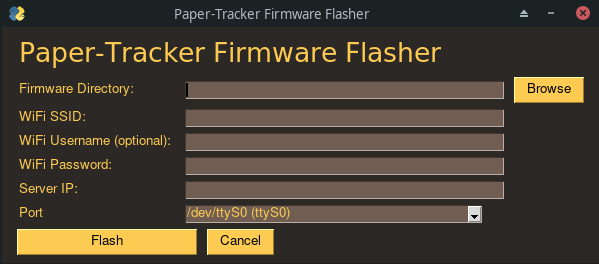
\includegraphics[width=\textwidth]{images/flasher/input.png}
	\centering
	\caption{Layout des Eingabe-Fensters}
	\label{fig:flasher-input}
\end{figure}

Das Programmier-Layout besteht lediglich aus einem Titel, einem Textfeld und einem Button.
Es ist in \autoref{fig:flasher-flash} dargestellt.
Im Textfeld soll der aktuelle Status angezeigt werden.
Der Button ist zum Schließen des Programms, sobald der Vorgang abgeschlossen ist.

\begin{figure}[htbp]
	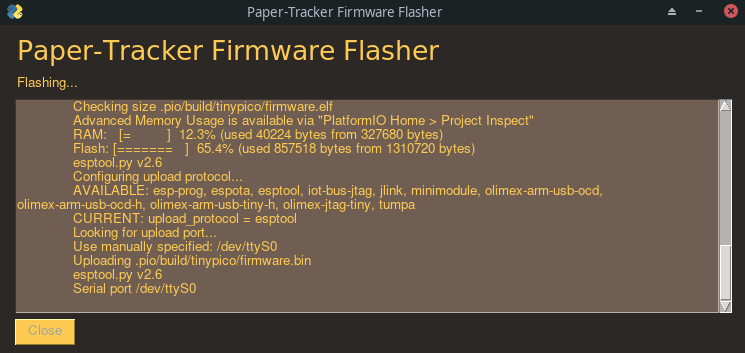
\includegraphics[width=\textwidth]{images/flasher/flash.png}
	\centering
	\caption{Layout des Programmier-Fensters}
	\label{fig:flasher-flash}
\end{figure}

Im Hauptteil des Skripts wird nun zuerst das Fenster mit dem Eingabe-Layout geöffnet.
Sobald der Button zum Start gedrückt wurde, werden die eingegebenen Werte ausgelesen.
Das Eingabe-Fenster wird geschlossen und das Programmier-Fenster mit dem entsprechendem Layout geöffnet.
Ist dieses offen, wird die Funktion zum Generieren der Konfigurationsdatei und die Funktion zum Programmieren des Trackers aufgerufen.
Im Textfeld des Layouts werden diese Schritte entsprechend dokumentiert.
Auch die Ausgabe des Programmierens wird im Textfeld abgebildet.
Nach dem Programmieren wird, je nach Kommandozeilenargument, die generierte Datei gelöscht.
Nun kann das Fenster und damit das gesamte Programm über den Schließen-Button geschlossen werden.

Tritt während dieses gesamten Vorgang ein Fehler auf, wird dieser entsprechend aufgefangen und die Fehlermeldung im Textfeld angezeigt.
Das Löschen der generierten Datei wird auch im Fehlerfall ausgeführt.

\subsection{Akkumulator}

Um \ref*{nf:akku} zu erfüllen, muss ein \gls{Akku} mit entsprechend großer Kapazität gewählt werden.
Zu diesem Zweck wird die Laufzeit des Trackers mit einem \gls{Akku} mit einer Kapazität von $850
mAh$ in verschiedenen Szenarien gemessen. Bei den Tests befindet sich der Tracker dauerhaft im
\enquote{Tracking}-Status, meldet also immer wieder die aktuelle Position an den Server. Dieser
Zustand wurde gewählt, da hier der Stromverbrauch am größten ist. Zu beachten ist jedoch, dass der
Tracker pro Zyklus (Aufwachen und Abholen eines Kommandos) immer nur einmal die \gls{WLAN}-Umgebung an den Server übermittelt. Wie in
\autoref{sec:tracker-lokalisierung} beschrieben, ist dies noch nicht unbedingt ausreichend, um den
Tracker zu lokalisieren.

Im ersten Test, dessen Ergebnis in
\autoref{fig:battery-runtime-quicktrack} in blau zu sehen ist, wurde dabei alle $10$ Sekunden die Position
des Trackers abgefragt.

\begin{figure}[htbp]
	\centering
	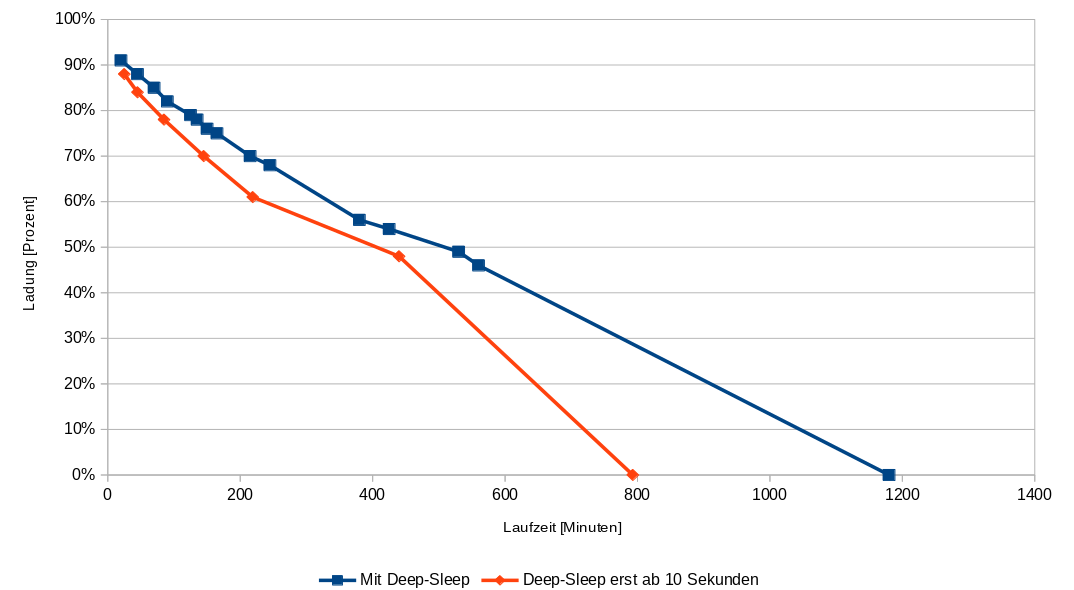
\includegraphics[width=.9\textwidth]{images/battery-runtime-quicktrack.png}
	\caption{Akkulaufzeit mit einem Tracking-Intervall von 10 Sekunden}
	\label{fig:battery-runtime-quicktrack}
\end{figure}

Beim ersten Test ist der Tracker nach dem Bearbeiten einer Aufgabe direkt in den \enquote{Deep-Sleep}
übergegangen. Beim zweiten Test (dargestellt in rot) erst dann, wenn die vom Server übermittelte Schlafdauer größer als $10$
Sekunden ist, was in diesem Test nie der Fall war. Wie deutlich zu sehen ist, kann durch das
sofortige Schlafen des Trackers eine um circa $400$ Minuten längere Laufzeit erreicht werden. Es ist
jedoch zu erwarten, dass der Tracker immer länger als $10$ Sekunden schläft, außer beim Einlernen
eines neuen Raumes. Bei dieser Operation ist vor allem die Reaktivität des Trackers wichtig, um
möglichst viele \glspl{AP} mit möglichst vielen Messungen zu erfassen. Daher wird die
Funktionalität, dass der Tracker sich nur in den \enquote{Deep-Sleep} begibt, wenn die Schlafdauer
$10$ Sekunden überschreitet, implementiert und die damit verbundene, geringere Laufzeit in Kauf
genommen.

\begin{figure}[htbp]
	\centering
	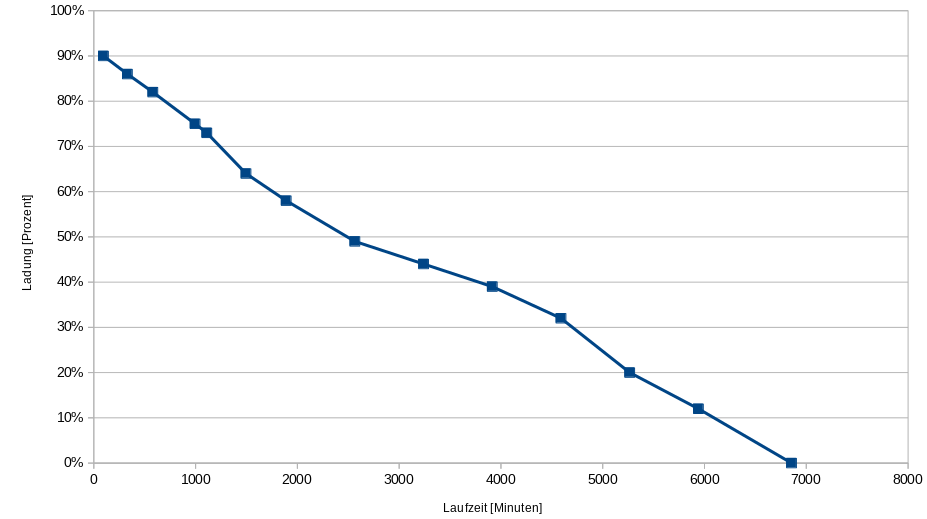
\includegraphics[width=.9\textwidth]{images/battery-runtime-slowtrack2.png}
	\caption{Akkulaufzeit mit einem Tracking-Intervall von 60 Sekunden}
	\label{fig:battery-runtime-slowtrack}
\end{figure}

In einem zweiten Szenario ist der Tracker alle $60$ Sekunden aufgewacht, um die aktuelle Position
zu ermitteln. Die Laufzeit des Trackers mit diesen Parametern ist in
\autoref{fig:battery-runtime-slowtrack} zu sehen. Wie zu sehen ist, skaliert die Laufzeit des
Trackers nahezu linear mit der Schlafdauer. Mit einer Schlafdauer von $60$ Sekunden konnte bereits
eine Laufzeit von mehr als 4 Tagen erreicht werden.

Daraus lässt sich schließen, dass sich \ref*{nf:akku} mit einem \gls{Akku} mit einer Kapazität von $850
mAh$ erfüllen lässt, indem der Tracker nicht den gesamten Tag aktiv ist oder das Tracking-Intervall
auf $120$ Sekunden erhöht wird. Da Dokumente üblicherweise nicht den gesamten Tag über getracked
werden müssen, sondern nur in den üblichen Arbeitszeiten, wird die Möglichkeit in den Server
implementiert, ebendiese zu definieren. So kann der Tracker meist den halben Tag inaktiv sein, am
Wochenende muss er gar nicht aufwachen.

\subsection{Sammeln von \glsentryshort{WLAN}-Daten}

Um die aktuelle \gls{WLAN}-Umgebung abzurufen und an den Server zu senden wird primär in das
Arduino-Framework eingebaute Funktionalität genutzt. Die durch das Framework bereitgestellte Klasse
\texttt{WiFi} bietet Methoden zur Abfrage aller \glspl{AP} inclusive deren \gls{BSSID},
\gls{SSID} und \gls{RSSI}.

\begin{lstlisting}[caption={Ausschnit aus der Firmware des Trackers -- Abrufen der \glsentryshort{WLAN}-Netzwerke},label={lst:wlan-firmware}]
std::vector<ScanResult> WIFI::getAllVisibleNetworks() {
  uint8_t visibleNetworkCount = WiFi.scanNetworks();
  std::vector<ScanResult> scanResults(0);
  for (auto i = 0; i < visibleNetworkCount; i++) {
    scanResults.emplace_back(WiFi.RSSI(i), WiFi.BSSIDstr(i), WiFi.SSID(i));
  }
  return scanResults;
}
\end{lstlisting}

In \autoref{lst:wlan-firmware} ist zu sehen, wie die Standardbibliothek genutzt wird. Die hier
erstellte Liste von Scanergebnissen wird, bevor sie zum Server gesendet wird, in mehrere Teile
geteilt. Diese enthalten jeweils fünf Scanergebnisse, damit die in
\autoref{sec:tracker-lokalisierung} beschriebene, maximale Größe eines \gls{UDP}-Paketes nicht
überschritten wird.

Die Arduino-\gls{API} gibt für die \texttt{WiFi.RSSI()}-Funktion an, dass diese eine Angabe in $dBm$
zurückliefert. (vgl. \cite{Arduino2020.1}) Durch diese Standardisierung kann jede
Entwicklungsplattform genutzt werden, die mit dem Arduino-Framework kompatibel ist, ohne dass die
Messung angepasst werden muss.

\subsection{\glsentryshort{API}-Client}

Um sich mit der vom Server angebotenen \gls{CoAP}-\gls{API} zu verbinden, wurde in der Firmware ein
entsprechender Client implementiert. Dieser nutzt eine erweiterte Version der \enquote{CoAP simple
library}\footnote{Original: \url{https://github.com/hirotakaster/CoAP-simple-library}} für die
Arduino-Plattform. Diese implementiert die Kommunikation mit einem \gls{CoAP}-Server, indem sie
Methoden zur Verfügung stellt, um Anfragen an einen Server zu senden und Antworten zu empfangen.

Die Klasse \texttt{APIClient}, welche in der Firmware genutzt wird, um die Kommunkation zu kapseln,
arbeitet mit Callbacks, um Antworten an Anfragen an den Aufrufer zurückzugeben. Dabei wird auch ein
Timeout-Mechanismus implementiert, welcher Anfragen abbricht, wenn für eine gewisse Zeit keine
Antwort empfangen wird. Dadurch wird verhindert, dass aufgrund der volatilen Natur von \gls{UDP} der
Tracker beliebig lange auf Antworten wartet und so sehr schnell den \gls{Akku} entleert.

Zusätzlich kümmert sich der \gls{API}-Client um die Serialisierung und Deserialisierung von
Nutzdaten in das \gls{CBOR}-Format.

\subsection{Serialisierung und Deserialisierung}

Wie in \autoref{par:tracker-schnittstelle} beschrieben, werden Nutzdaten zwischen Server und Tracker
mit \gls{CBOR} codiert ausgetauscht. Dieses Format ist besonders performant und leichtgewichtig und
daher optimal für den Einsatz im \gls{IoT} geeignet. Implementiert wurde ein System zur
Serialisierung und Deserialisierung auf Basis der \enquote{libCBOR}-Bibliothek \footnote{Siehe
\url{https://github.com/ssilverman/libCBOR}}. Das entwickelte System ermöglicht es, sehr schnell und
einfach Entitäten zu \gls{CBOR} zu serialisieren und zu deserialiseren.

\begin{lstlisting}[caption={Beispiel zur Deserialisierung von \glsentryshort{CBOR} mit den
entwickelten Helferklassen},label={lst:cbor-deserialiserung}]
class Command {
private:
	CBORUint16 sleepTimeSec{"sleep_time_sec"};
	CBORUint8 type{"type"};
public:
	bool fromCBOR(uint8_t* buffer, size_t bufferSize) {
		auto cbor = CBORParser(buffer, bufferSize);
		if (!cbor.isWellformedModel()) { return false; }

		while(cbor.advance()) {
			auto key = cbor.findNextKey();
			if (key == nullptr) { continue; }

			if (type.matchesKey(key)) {
				type.deserializeFrom(cbor);
			} else if (sleepTimeSec.matchesKey(key)) {
				sleepTimeSec.deserializeFrom(cbor);
			}
		}

		return true;
	}
};
\end{lstlisting}

So ist in \autoref{lst:cbor-deserialiserung} der vollständige, zur Deserialisierung eines Befehls
vom Server an den Client nötige Code gezeigt. Einzig die Fehlerbehandlung wurde zur
Übersichtlichkeit entfernt. Für die Implementierung der Bibliothek wurden eigene Typen entwickelt,
die Basisdatentypen wiederspiegeln (\texttt{CBORUint8}, \texttt{CBORInt16}, \texttt{CBORString},
...) und die Serialisierung und Deserialisierung in sich kapseln.

\section{Backend-Server}

\subsection{Verwendete Technologien} \label{sec:impl-server-technology}

Die grundlegend verwendete Technologie für den Backend-Server ist die Programmiersprache \enquote{Go}.
Go wurde ausgewählt, da es eine einfach zu verstehende Programmiersprache ist, die optimiert für Server-Anwendungen ist (vgl. \cite{Weigend2019}).
Zudem sind alle am Projekt beteiligten Personen schon mit der Sprache vertraut.

Go stellt eine gute Standardbibliothek zur Verfügung, die an vielen Stellen verwendet wird.
Trotzdem werden zusätzlich einige externe Bibliotheken verwendet.
Diese dienen hauptsächlich dazu, die externen Schnittstellen (\gls{HTTP} und \gls{CoAP}) mit den dazugehörigen Datenformaten zur Verfügung zu stellen.
Auch werden Bibliotheken für ein einfacheres Testing verwendet.

Im Folgenden sind die verwendeten Bibliotheken aufgelistet:
\begin{description}
	\item[pflag (https://github.com/spf13/pflag)] \hfill \\
		\enquote{pflag} wird zum Angeben und Parsen von Kommandozeilenargumenten verwendet. Es ist kompatibel mit \enquote{viper}.
	\item[viper (https://github.com/spf13/viper)] \hfill \\
		Für die Konfiguration des Servers wird \enquote{viper} verwendet. Es kann Konfigurationen aus \enquote{pflag}, Dateien und mehr einlesen.
	\item[logrus (https://github.com/sirupsen/logrus)] \hfill \\
		\enquote{logrus} ist ein strukturiertes Logging-Tool, das für jegliche Logs innerhalb des Servers verwendet wird.
	\item[gorm (https://github.com/jinzhu/gorm)] \hfill \\
		\enquote{gorm} ist ein \gls{ORM} Framework, das die Datenbankanbindung für den Server zur Verfügung stellt.
	\item[Gin (https://github.com/gin-gonic/gin)] \hfill \\
		\enquote{Gin} ist ein HTTP Framework, das Routing, Parameter-Matching, etc. übernimmt. Zudem kann es standardmäßig \gls{JSON} verstehen.
	\item[go-coap (https://github.com/go-ocf/go-coap)] \hfill \\
		\enquote{go-coap} ist ein \gls{CoAP} Framework, das hauptsächlich das Routing übernimmt. Einige weitere Aufgaben, die z.B. \enquote{Gin} übernimmt, müssen selbst programmiert werden.
	\item[go-codec (https://github.com/ugorji/go)] \hfill \\
		\enquote{go-codec} stellt die Codierung für \gls{CBOR} zur Verfügung.
	\item[now (https://github.com/jinzhu/now)] \hfill \\
		\enquote{now} stellt Hilfsfunktionen für Zeitberechnungen zur Verfügung.
	\item[stats (https://github.com/montanaflynn/stats)] \hfill \\
		\enquote{stats} stellt einige mathematische Funktionalitäten für statistische Berechnungen zur Verfügung.
	\item[xlsx (https://github.com/tealeg/xlsx)] \hfill \\
		Mit \enquote{xlsx} können Dateien im \gls{XLSX} Dateiformat erstellt, bearbeitet und gelesen
		werden. Im Server wird sie für das Erstellen des Excel-Exports genutzt.
	\item[gomail (https://github.com/go-gomail/gomail)] \hfill \\
		\enquote{gomail} wird verwendet, um E-Mails verschicken zu können.
	\item[ginkgo (https://github.com/onsi/ginkgo)] \hfill \\
		Mit \enquote{ginkgo} können Tests in \gls{BDD} Technik geschrieben werden.
	\item[gomega (https://github.com/onsi/gomega)] \hfill \\
		\enquote{gomega} ist eine Matching Library, die zu \enquote{ginkgo} gehört. Sie stellt Vergleiche zwischen erwarteten Werten und tatsächlichen Werten zur Verfügung.
	\item[GoMock (https://github.com/golang/mock)] \hfill \\
		\enquote{GoMock} ist ein Mocking Framework, das für verschiedene Tests verwendet wird.
\end{description}

Als Datenbank wird in Kombination mit \enquote{gorm} eine \enquote{SQLite} verwendet.
Der große Vorteil ist, dass eine SQLite Datenbank eine einfache Datei ist und kein externer Server aufgesetzt werden muss.
Dies vereinfacht vor allem die Entwicklung.
Zum Beispiel ist ein einfaches Zurücksetzen der Daten durch ein Löschen der Datei möglich.

In einem späteren Einsatz des Paper-Trackers können dank der \enquote{gorm} Bibliothek auch andere
Datenbanken verwendet werden, die eher für einen dauerhaften und sichereren Einsatz vorgesehen sind.
Möglich sind dafür \enquote{MySQL}, \enquote{PostgreSQL}, \enquote{Microsoft SQL Server} und wie erwähnt SQLite.
Im Code des Servers muss hierfür lediglich eine erweiterte Konfiguration ermöglicht werden. (vgl. \cite{Jinzhu2020})

\subsection{\glsentryfull{REST}-Schnittstelle}

Die \gls{REST}-Schnittstelle zur Anbindung der App wurde wie in \autoref{par:app-schnittstelle}
beschrieben implementiert.
Dabei wurden alle Endpunkte entsprechend umgesetzt.
Wie in \autoref{sec:impl-server-technology} erwähnt, wird das Gin-Framework als
\gls{HTTP}-Router und zum Serialisieren sowie Deserialisieren der Nutzdaten verwendet.
Das Framework ermöglicht es, für jeden \gls{REST}-Endpunkt, also für jede Kombination aus
\gls{HTTP}-Verb und \gls{URL} eine sogenannte Handler-Funktion zu definieren. Diese wird aufgerufen,
wenn eine Anfrage an die entsprechende Ressource getätigt wird. Die Handler-Funktionen parsen
zunächst die Anfragedaten in entsprechende Go-Strukturen. Im Anschluss werden eine oder mehrere
Manager-Funktionen aufgerufen, welche die Geschäftslogik enthalten. Das Ergebnis dieses Aufrufes
wird dann von der Handler-Funktion in das Zielformat, in diesem Fall \gls{JSON}, serialisiert und an
den Aufrufer gesendet.

\subsection{\glsentryfull{CoAP}-Schnittstelle}

Die \gls{CoAP}-Schnittstelle für die Tracker wurde grundsätzlich wie in
\autoref{par:tracker-schnittstelle} beschrieben implementiert. Es wurde allerdings ein weiterer
Endpunkt hinzugefügt: Über den Pfad \texttt{/tracker/status}, welcher mit dem Verb \texttt{POST}
angesprochen wird, kann der Tracker aktuelle Statuswerte, wie beispielsweise die aktuelle
Akkuladung, an den Server übermitteln. Diese Statuswerte werden bei aktivem Tracking in den
Scanergebnis-Paketen übermittelt. Wenn der Tracker sich jedoch im Leerlauf befindet, sendet der
Server periodisch Status-Kommandos an den Tracker, sodass auch hier der Ladezustand des \gls{Akku}s, sowie
die verbleibende Restladung aktualisiert werden können.

\subsection{Tracker-Lokalisierung} \label{sec:tracker-lokalisierung}

Wie in \autoref{sec:tracking-hardware} beschrieben, wird die Lokalisierung der Tracker mit einem
Score-basierten System durchgeführt.

Dazu werden zunächst Scanergebnisse vom jeweiligen Tracker gesammelt und dann ausgewertet. Da die
Datengröße der Scanergebnisse je nach Anzahl der vom Tracker sichtbaren \gls{WLAN}-Netzwerke zu
groß für ein einzelnes \gls{UDP}-Paket ist\footnote{Im Arduino-Framework gibt es eine
Limitierung von 1446 Bytes für die Größe eines \gls{UDP}-Paketes. (vgl. \cite{Arduino2020})}, wurde
das \gls{API} so gestaltet, dass die Ergebnisse in mehreren Paketen an den Server übermittelt werden
können. Dazu berechnet der Tracker im Voraus, in wie viele Pakete die Scanergebnisse geteilt werden
müssen. Diese Zahl, sowie eine für den Ergebnissatz einheitlicher, zufällig erzeugter \gls{ID} sind
jedem Teilpaket angehängt. So kann der Server erkennen, ob alle Ergebnisse empfangen wurden und
diese dann verwenden. Dass nicht alle Pakete eines Ergebnissatzes beim Server angekommen sind, ist
dadurch erkennbar, dass eine andere \gls{ID} empfangen wird. In diesem Fall werden alle vom
vorherigen Paket empfangenen Scanergebnisse verworfen und die neuen Pakete gespeichert.
\TODO{Das hier kann vielleicht zu CoAP-Schnittstelle verschoben werden}

Sobald ein vollständiger Ergebnissatz empfangen wurde, wird aus diesem ein Score für jeden Raum
ermittelt. Dieser Score ist eine Zahl, deren Wert größer wird, je besser die gemessene
\gls{WLAN}-Umgebung mit der gelernten übereinstimmt.

\begin{lstlisting}[caption={Pseudocode-Beschreibung der Scoring-Funktion},label={lst:scoring},tabsize=2]
# Berechnet den Score für ein Scanergebnis und einen Raum
#
# rssi ist das aktuelle Scanergebnis des Trackers
# room enthält die zuvor gelernten Scandaten
func getScoreForScanResultAndRoom(rssi, room) float {
	score := 0.0
	rssiFactor := math.Abs(rssi / 100.0)

	if rssi <= room.Maximum && rssi >= room.Minimum {
		score += inMinimumMaximumFactor * rssiFactor
	}
	if rssi < room.ThirdQuartile && rssi > room.FirstQuartile {
		score += inQuartilesFactor * rssiFactor
	}
	if isInRange(rssi, room.Mean, rangeForMean) {
		distance := math.Abs(room.Mean - rssi)
		score += math.Abs(distance-rangeForMean) * inMeanRangeFactor * rssiFactor
	}
	if isInRange(rssi, room.Median, rangeForMedian) {
		distance := math.Abs(room.Median - rssi)
		score += math.Abs(distance-rangeForMedian) * inMedianRangeFactor * rssiFactor
	}
	return score
}
\end{lstlisting}

\autoref{lst:scoring} zeigt einen Teil des Scoring-Algorithmus. Dieser Teil wird für jeden Raum und
jedes Scanergebnis ausgeführt. In den vier \texttt{if}-Zweigen werden jeweils Punkte dafür vergeben,
dass das Scanergebnis in einem bestimmten Bereich liegt. Die Zweige sind nach ihrer Signifikanz
geordnet. So wird ein Scanergebnis, welches im Bereich des vorher gelernten Minimums und Maximums
liegt, mit wenigen Punkten \enquote{belohnt}, während es viele Punkte bekommen kann, wenn es sehr
nahe am arithmetischen Mittel liegt.

Die genaue Punkteverteilung ist konfigurierbar, um den Algorithmus möglichst offen für
unterschiedliche \gls{WLAN}-Umgebungen zu machen. Die Standardwerte der Parameter
\texttt{inMinimumMaximumFactor}, \texttt{inQuartilesFactor}, \texttt{inMeanRangeFactor} und
\texttt{inMedianRangeFactor} wurden experimentell für das \gls{WLAN}-Netz der \gls{DHBW} ermittelt und liegen
bei $1$, $5$, $5$ und $5$.

Zu beachten ist, dass ein Einschluss in Minimum/Maximum und erstem und drittem Quartil dem
Scanergebnis eine fixe Punktzahl gewährt, während beim Median und Mittel jeweils mit Abständen
kalkuliert wird. So bekommt ein Ergebnis, welches näher an einem der beiden Werte liegt, eine
größere Punktzahl. Die Punktzahl skaliert dabei linear zum Abstand.

Der \texttt{rssiFactor} in Zeile 7 wird verwendet, um weiter entfernte \glspl{AP} weniger in die
Berechnung mit einfließen zu lassen. Da die von den Trackern ermittelte \gls{RSSI} nicht exakt ist
und oft auch ohne ein Bewegen des Trackers um wenige $dBm$ schwankt, wird so verhindert, dass eine
Schwankung von beispielsweise $-80dBm$ auf $-82dBm$ die gleiche Auswirkung hat, wie eine gleichgroße
Schwankung eines \gls{AP}s mit deutlich besserem Empfang.

Die Scores für jede \gls{BSSID}, also auch für jedes Scanergebnis, werden dann pro Raum addiert,
wobei eine eingelernte \gls{BSSID}, für welche kein Scanergebnis existiert, mit $-10$ Punkten
\enquote{bestraft} wird. Nun liegt für jeden Raum ein Gesamt-Score vor, anhand dessen der passendste
Raum ausgewählt werden kann. Dies ist der Raum mit dem größten Score.

Aufgrund der bereits beschriebenen Schwankungen beim Scannen der \glspl{AP} wird dieses Scoring
jedoch mehrfach (Standardfall: dreifach) durchgeführt und der beste Raum anhand des arithmetischen
Mittels der Scores ausgewählt. Dies verlängert einen Lokalisierungsvorgang pro Messung um etwa
$5-15$ Sekunden, was allerdings kein Problem ist, da die Lokalisierung nicht in Echtzeit
durchgeführt werden muss.

Damit kein Raum ausgewählt wird, in dem der Tracker nicht liegt, muss jeder Raum einen Schwellwert
erreichen, um in die Auswahl aufgenommen zu werden. Dieser Schwellwert ist auf $600$ gesetzt, was im
Umfeld der \gls{DHBW} zu guten Ergebnissen geführt hat. Dieser Wert ist jedoch, wie die restlichen
Scoring-Parameter, durch den Nutzer konfigurierbar.

\subsection{Daten-Export}

In diesem Kapitel wird die Implementierung des Datenexports in eine Excel-Datei näher erläutert.
Dieser besteht aus größtenteils zwei Unterpunkten: Dem Sammeln und Aufbereiten der Daten für den
Export und das Schreiben der Excel-Datei selbst.
Beides wird zusammengefasst im \enquote{ExportManager} durchgeführt.

Um die Daten für den Export zu sammeln, nutzt der \enquote{ExportManager} einige andere Manager:
\enquote{WorkflowTemplateManager}, \enquote{WorkflowExecManager} und \enquote{RoomManager}.
Über diese können alle benötigten Daten abgefragt werden.
Zuerst werden alle Templates abgefragt.
Für jedes Template werden alle verfügbaren Ausführungen des Templates angefordert.
Weiter wird für jeden Schritt in einem Template/einer Ausführung Informationen über die Schritte und die den Schritten
zugewiesenen Räume abgefragt.
Während die Daten gesammelt werden, werden auch einige Metriken erfasst: Die Anzahl Ausführungen pro Template,
wie viele Ausführungen beendet wurden und wie lange eine durchschnittliche Ausführung gebraucht hat.

Nachdem alle grundlegenden Daten gesammelt wurden, wird nochmals durch alle Templates iteriert und diese nach Revisionen sortiert.
Dies bedeutet, dass alle Templates zusammen gruppiert werden, die die gleiche ursprüngliche Revision haben.
Die ursprüngliche Revision selbst wird auch mit gruppiert.
Damit sind alle Daten entsprechend gesammelt und aufbereitet, um exportiert zu werden.

Für den Export selbst wird, wie schon in \autoref{sec:impl-server-technology} angemerkt, die Bibliothek \enquote{xlsx} verwendet.
Die Entscheidung, diese Bilbiothek zu nutzen, wurde getroffen, da sie eine simple Schnittstelle hat und regelmäßig aktualisiert wird
(Stand 20. April 2020: Letzte Aktualisierung vor 24 Tagen \cite{tealeg2020}).

\enquote{xlsx} arbeitet mit Pointern auf Objekte verschiedener Typen, die jeweils ein Objekt in Excel wiederspiegeln.
So gibt es zum Beispiel Objekte für eine Excel-Datei, ein Sheet in einer Datei und eine Zelle eines Sheets.
Eine Datei kann über eine Funktion der Bibliothek erstellt werden, ein Sheet kann über das Datei-Objekt erstellt werden
und ein Zell-Objekt über das Sheet-Objekt.

Für den Excel-Export des Paper-Trackers wird zunächst eine neue Datei erstellt.
Diese ist nur im Hauptspeicher vorhanden und wird nicht auf die Festplatte geschrieben.
Weiter wird für jedes Workflow Template ein Sheet erstellt.
In dieses Sheet werden als Tabelle alle Ausführungen dieses Templates mit Informationen zu den Schritten geschrieben.
Dies geschieht schon während des Sammelns der Daten.
Ein Beispiel für ein solches Sheet ist in \autoref{fig:export-template} zu sehen.

\begin{figure}[htbp]
	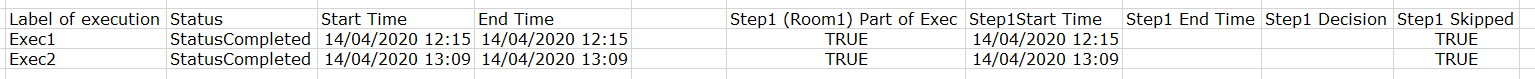
\includegraphics[width=\textwidth]{images/export_template.png}
	\centering
	\caption{Template-Sheet eines Excel-Exports}
	\label{fig:export-template}
\end{figure}

Für die Übersicht der Revisionen wird zusätzlich ein separates Sheet erstellt.
In dieses werden nach dem Aufbereiten der Daten in einer Tabelle die verschiedenen ursprünglichen Revisionen
mit ihren folgenden Revisionen gelistet.
Hier werden auch die erfassten Metriken dargestellt.
Dies resultiert in dem in \autoref{fig:export-orig-revisions} dargestellten Sheet.

\begin{figure}[htbp]
	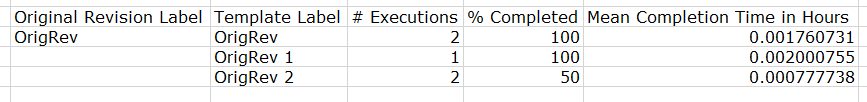
\includegraphics[width=\textwidth]{images/export_orig_revisions.png}
	\centering
	\caption{Ursprüngliches Revisionen-Sheet eines Excel-Exports}
	\label{fig:export-orig-revisions}
\end{figure}

Die daraus entstandene Excel-Datei ist immernoch nur im Hauptspeicher vorhanden
und muss auch nicht auf die Festplatte geschrieben werden.
Das Objekt der Datei kann auf ein \enquote{io.Writer}-Interface,
das in der Standardbibliothek von Go enthalten ist, schreiben.
Dadurch kann das Objekt direkt in die Antwort der \gls{REST}-Schnittstelle die Datei schreiben.

\subsection{Tests}

Wie in allen Software-Projekten ist es wichtig, den Paper-Tracker zu testen.
Dabei spielt vor allem der Backend-Server ein große Rolle, da dieser die meiste Geschäftslogik implementiert.

Alle für den Server existierenden Tests sind automatisierte Tests, die einzelne Einheiten des Codes testen.
Vor allem werden die Manager getestet, da diese letztendlich die Geschäftslogik beinhalten.
Dafür werden verschiedene Bibliotheken verwendet.
Die \enquote{ginkgo}-Bibliothek stellt Funktionen zur Verfügung, um die Tests zu definieren
und Code vor/nach den Tests auszuführen.
Mit Hilfe von \enquote{gomega} können Ergebnisse der Tests mit zu erwartenden Ergebnissen verglichen werden.
Sie stellt neben den einfachen Vergleichen auch Vergleiche für Fehlertypen, komplexe verschachtelte Datenstrukturen,
Listen und mehr.

Damit die einzelnen Einheiten des Servers getrennt voneinander getestet werden können, wird zusätzlich die
\enquote{gomock} Bibliothek verwendet.
Diese ermöglicht es, Stellvertreterobjekte für in diesem Fall Manager und Repositories zu erstellen.
Die Stellvertreterobjekte können dann für jeden einzelnen Testfall mit zu erwarteten Parametern und einem Rückgabewert
konfiguriert werden.
Da \enquote{gomock} nur aus Interfaces Stellvertreterobjekte erstellen kann, müssen für alle Manager
und Repositories eigene Interfaces erstellt werden.
Deshalb gibt es, im Gegensatz zum Entwurf, für jeden Manager ein Interface und eine Implementierungsklasse.
Für die Tests wird dann die Instanz des Singletons auf ein Stellvertreterobjekt gesetzt.

Mit diesen Techniken wurden einige Tests für die Manager-, Modell- und Utilities-Klassen geschrieben.
Es sind somit ca. $20\%$ der Manager, ca. $27\%$ der Modelle und ca. $68\%$ der Utilities getestet.
Leider ist dies noch nicht ausreichend für eine gute Testabdeckung.
Vor allem, um komplexe Konstrukte wie den Fortschritt einer Workflow Ausführung zu testen, wäre um einiges mehr Zeit erforderlich
gewesen.

\section{App}

In diesem Kapitel wird die technische Umsetzung der App für Mobilgeräte beschrieben.

\subsection{Verwendete Technologien}

Zur Programmierung der App wurden die Programmiersprache Dart und das Framework Flutter verwendet.
Ein großer Vorteil dieser Kombination ist, dass Anwendungen sowohl für Android als auch für iOS
kompiliert werden können, ohne den Quellcode anpassen zu müssen. Auch eine Laufzeitumgebung für
Desktopcomputer unter Windows, macOS und GNU/Linux befindet sich aktuell im Teststadium, sodass die
Paper-Tracker App gegebenenfalls auch auf Arbeitsplatzrechnern verwendet werden kann.

Auch für das Erstellen der App wurden einige Bibliotheken verwendet, die die Entwicklung vereinfachen.
Vor allem werden zum Beispiel Bibliotheken verwendet, um die Kommunikation mit dem Backend-Server zu ermöglichen.
Die verwendeten Bibliotheken sind im Folgenden aufgelistet:
\begin{description}
	\item[http (https://pub.dev/packages/http)] \hfill \\
		\enquote{http} ist eine Bibliothek, die es ermöglicht, asynchron \gls{HTTP}-Anfragen durchzuführen. Die Bibliothek wird dafür verwendet, um mit dem Backend-Server zu kommunizieren.
	\item[json\_annotation (https://pub.dev/packages/json\_annotation)] \hfill \\
		Mit \enquote{json\_annotation} kann über Annotationen im Programmcode eine Serialisierung zu \gls{JSON} und Deserialisierung von \gls{JSON} für Datenklassen generiert werden.
	\item[shared\_preferences (https://pub.dev/packages/shared\_preferences)] \hfill \\
		Durch die \enquote{shared\_preferences} Bibliothek können einfache Konfigurationen als Schlüssel-Wert-Paare abgespeichert werden. Dies wird für die \gls{URL} des Backend-Servers verwendet.
	\item[material\_design\_icons (https://pub.dev/packages/material\_design\_icons\_flutter)] \hfill \\
		\enquote{material\_design\_icons} stellt zusätzliche Material\footnote{Eine Designsprache von
			Google, die in fast allen Google-Produkten eingesetzt wird und auf Minimalismus setzt.
			\cite{Google2020}}-Icons zur Verfügung. Dies ist notwendig, da die standardmäßig verfügbaren Icons in Flutter nicht ausreichend sind.
	\item[fluttertoast (https://pub.dev/packages/fluttertoast)] \hfill \\
		Mit \enquote{fluttertoast} können kleine Pop-ups dargestellt werden, die dem Nutzer der App einfach und schnell Feedback zu einer Aktion geben können.
	\item[url\_launcher (https://pub.dev/packages/url\_launcher)] \hfill \\
		Mit Hilfe von \enquote{url\_launcher} können \gls{URL}s im Browser des Smartphones geöffnet
		werden. Für den Paper-Tracker wird dies zum Download des Daten-Exports verwendet.
	\item[intl (https://pub.dev/packages/intl)] \hfill \\
		Die \enquote{intl}-Bibliothek wird für das Formatieren von Daten und Uhrzeiten verwendet. Zudem kann sie für die Übersetzung der App in andere Sprachen verwendet werden.
\end{description}

\subsection{Struktur der App}

Die Struktur der App teilt sich in fünf Teile auf.
Der erste Teil bildet die Hauptdatei, in der die App gestartet wird, sowie zusätzlich eine Konfigurations- und eine
Hilfsfunktions-Datei.
In der Hauptdatei wird neben dem Start der App auch das Design (hauptsächlich die zu verwendenden Farben) und die
Navigation aufgesetzt.
Die Navigation wird weiter unten detailiert erläutert.

Weiter sind im Unterordner \enquote{model} alle Modell-Klassen, die auch für den Server verwendet werden, vorhanden.
Für diese wird mit Hilfe der \enquote{json\_annotation} Bibliothek Code für die Serialisierung zu \gls{JSON} und die
Deserialisierung von \gls{JSON} generiert.

Um Daten dieser Modelle vom Server abzurufen, werden verschiedene Klienten-Klassen aus dem \enquote{client}-Ordner verwendet.
Es gibt einen grundlegenden Klienten, welcher eine Verfügbarkeitsabfrage und Anfragen an den Server zur Verfügung stellt.
Dieser verwendet die konfigurierte Server \gls{URL}.
Die Anfragen werden über die \enquote{http} Bibliothek ausgeführt.
Die weiteren Klienten (z.B. \enquote{RoomClient}) verwenden den grundlegenden Klienten und stellen Funktionen direkt im Bezug
auf die zugehörige Klasse des Klienten zur Verfügung.
So können über den \enquote{RoomClient} zum Beispiel alle Räume abgefragt werden.
Diese Klienten führen dann die Konvertierung von und zu \gls{JSON} durch.

Im \enquote{pages} Unterordner sind alle anzuzeigenden Seiten der App untergebracht.
Dies sind zum Beispiel die Hauptübersichtsseite oder die Detailseite für einen Raum.
Auf diesen Seiten werden sogenannte \enquote{Widgets} verwendet, aus denen letztendlich das Layout und der Inhalt einer
Seite zusammengesetzt werden.
Neben den durch die Standardbibliothek und weiteren Bibliotheken bereitgestellten Widgets werden auch selbst programmierte verwendet.
Diese befinden sich im \enquote{widgets} Unterordner.
Der Aufbau einer Seite und eines Widgets sind weiter unten näher erklärt.

\subsection{Routing}

Unter Routing versteht man die Navigation innerhalb der App auf verschiedene Routen und damit im Falle der Paper-Tracker
App auf verschiedene Seiten.
Für das Routing wird in der App die Standard-Klasse \enquote{MaterialApp} verwendet.
Dieser wird eine Zuordnung von einer Route zu einer Seite in Form einer Zeichenkette mitgegeben.

In der kompletten App kann dann über \enquote{Navigator.of(context)} auf die Navigation zugegriffen werden.
Der Kontext ist in jeder zur App zugehörigen Seite und Widget vorhanden.
Die Navigation bietet die folgenden wichtigen Funktionalitäten:
Mit \enquote{pushNamed} kann über die zuvor in der Zuordnung definierte Route auf die dazugehörige Seite navigiert werden.
Diesem Funktionsaufruf können auch Parameter mitgegeben werden, die von der geöffneten Seite verwendet werden können.
Über \enquote{pop} kann die zuletzt geöffnete Seite wieder geschlossen werden.
Dabei wird die zuvor geöffnete Seite wieder angezeigt oder bei der letzten Seite die App geschlossen.

Für die Paper-Tracker App gibt es für jede Seite eine eigene Route.
Diese Route ist in der Klasse der Seite statisch definiert.
Somit kann jederzeit in der App auf eine beliebige Seite navigiert werden.

Einige Beispiele für die Navigation innerhalb der App sind in \autoref{lst:app_navigation} aufgeführt.

\begin{lstlisting}[caption={Beispiele für die Navigation innerhalb der App},label={lst:app_navigation},tabsize=2]
// Navigiere zur ConfigPage
Navigator.of(context).pushNamed(ConfigPage.Route);

// Navigiere zur RoomPage mit der ID des Raumes als Parameter
Navigator.of(context).pushNamed(RoomPage.Route, arguments: room.id);

// Schließe die aktuelle Seite und kehre zur vorherigen zurück
Navigator.of(context).pop();
\end{lstlisting}

\subsection{Seiten}

Insgesamt beinhaltet die App elf verschiedene Seiten:
\begin{enumerate}
	\item InitPage
	\item ConfigPage
	\item ServerConfigPage
	\item MainPage
	\item WorkflowExecPage
	\item WorkflowTemplatePage
	\item RoomPage
	\item TrackerPage
	\item LearningPage
	\item StartExecPage
	\item TutorialPage
\end{enumerate}
Der Großteil der Seiten spiegelt Seiten aus dem Entwurf der App wieder.
Zwei dieser Seiten sind in \autoref{fig:app_pages} dargestellt.
Weitere Seiten, wie die \enquote{InitPage} oder \enquote{ConfigPage}, werden nur als Weiterleitung oder für nicht im
Entwurf beinhaltete Funktionen genutzt.

\begin{figure}[htbp]
	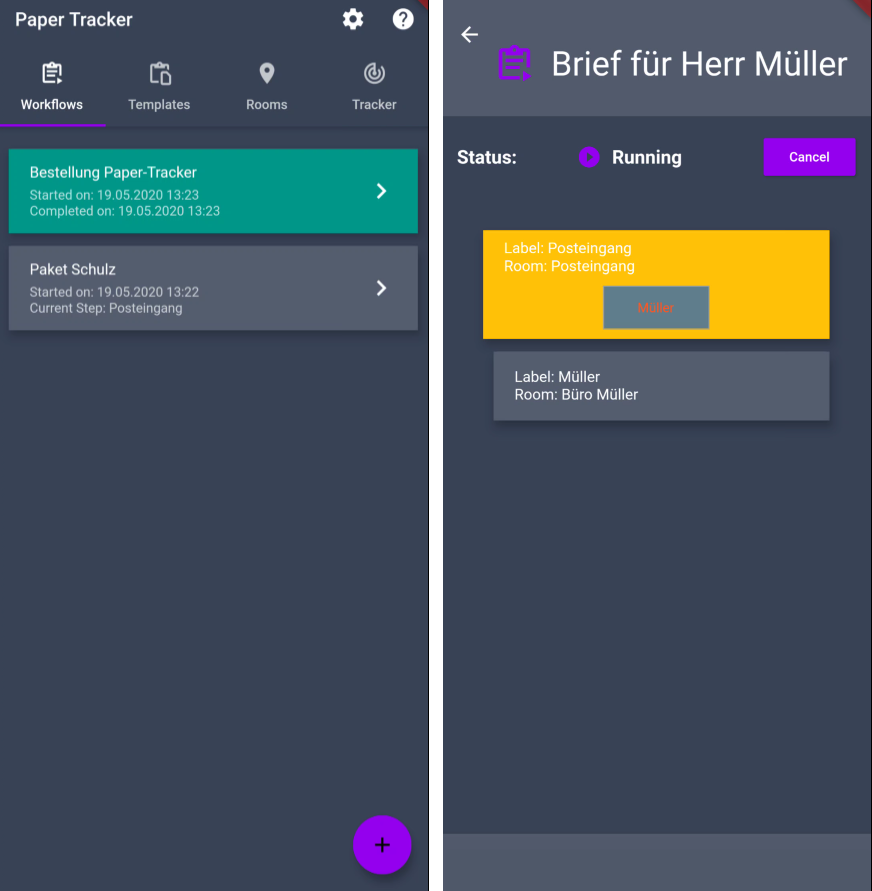
\includegraphics[height=300px]{images/app.png}
	\centering
	\caption{Umsetzung des App Entwurfs}
	\label{fig:app_pages}
\end{figure}

Eine Seite selbst ist, wie bereits erwähnt, aus verschiedenen Widgets zusammengesetzt.
Für alle Seiten der Paper-Tracker App wird dafür als Grundlage das \enquote{Scaffold}-Widget verwendet.
Dieses bietet eine \enquote{AppBar} als Titel für die Seite und als Container für z.b. eine Zurück-Schaltfläche.
Auch kann über das \enquote{Scaffold}-Widget ein \enquote{FloatingActionButton} für die Seite verwendet werden.
Dieser wird für die \enquote{WorkflowExecPage} zum Erstellen einer neuen Ausführung und für die \enquote{RoomPage}
zum Erstellen eines neuen Raums benötigt.
Der eigentliche Inhalt der Seite wird dem \enquote{Scaffold} als Parameter mitgegeben.
Ein \enquote{Scaffold} mit Titel und \enquote{FloatingActionButton} ist in \autoref{fig:app_scaffold} dargestellt.

\begin{figure}[htbp]
	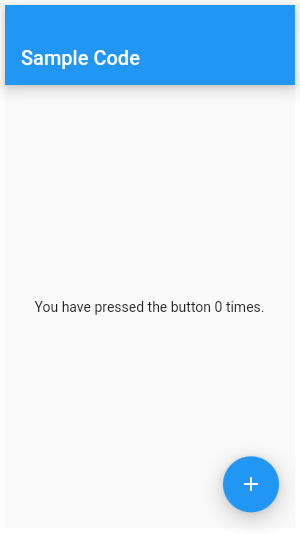
\includegraphics[height=300px]{images/scaffold.png}
	\centering
	\caption{Scaffold-Widget}
	\small Quelle: \url{https://api.flutter.dev/flutter/material/Scaffold-class.html}
	\label{fig:app_scaffold}
\end{figure}

Der eigentliche Inhalt der Seiten variiert stark und besteht gemischt aus Widgets der Standardbibliothek, weiteren Bibliotheken
und eigenen Widgets.
Die Widgets bauen letztendlich eine Baumstruktur auf.
Eine besonders wichtige Rolle spielt dabei unter anderem das \enquote{FutureBuilder} Widget.

Der \enquote{FutureBuilder} erlaubt einer Seite asynchron auf ein Ergebnis eines \enquote{Future}\footnote{Ein Future repräsentiert in Dart das Ergebnis
einer asynchronen Ausführung. Dabei kann ein Future entweder das Ergebnis selbst oder im Fehlerfall einen Fehler zurückgeben. \cite{dart2020}}
 zu warten.
Futures werden bei allen Anfragen über die Klienten an den Server verwendet, da die Ergebnisse der Netzwerkanfragen asynchron sind.
Welche Widgets letztendlich durch den \enquote{FutureBuilder} angezeigt werden, entscheidet sich in einer Funktion,
die dem Widget mitgegeben wird.
In dieser Funktion kann je nachdem, ob ein Ergebnis vorhanden ist und ob das Ergebnis die erwarteten Daten oder
ein Fehler ist, entsprechend weitere Widgets gebaut werden.
Ein Beispiel ist in \autoref{lst:app_futurebuilder} aufgelistet.

\begin{lstlisting}[caption={Beispiel für die Verwendung des \enquote{FutureBuilder}},label={lst:app_futurebuilder},tabsize=2]
@override
Widget build(BuildContext context) {
	return FutureBuilder(
		future: RoomClient.getAllRooms(),
		builder: (context, snapshot) {
			if (snapshot.hasData) {
        // Zeige eine Raumliste bei erfolgreichem Abfragen der Daten an
				return RoomList(snapshot.data);
			} else if (snapshot.hasError) {
        // Zeige einen Fehler bei Auftreten an
        return Center(child: Text("${snapshot.error}"));
      }
      // Falls es noch kein Ergebnis gibt, zeige einen Ladekreis an
			return CircularProgressIndicator();
		},
	);
}
\end{lstlisting}

\FloatBarrier
\subsection{Widgets}

Wie bereits erwähnt, wurden einige Widgets, die auf den Seiten der App verwendet werden, selbst programmiert.
Dies hilft dabei duplizierte Konstellationen von Widgets auf verschiedenen Seiten zu verringern, indem man diese
verallgemeinert und als eigenes Widget zur Verfügung stellt.
Auch können in diesen Widgets bestimmte Design-Formatierungen gemacht werden, die dann an dieser Stelle zentral verwaltet
werden können.
Allgemein können die eigenen Widgets in drei Kategorien aufgeteilt werden:
Dialoge, Listen und allgemeine Widgets.

Dialoge beinhalten teilweise generalisierte und teilweise spezialisierte Dialoge, die von den Seiten aus aufgerufen werden können.
Ein Beispiel für einen generalisierten Dialog ist ein einfacher \enquote{Bestätigen} Dialog.
Ein spezialisierter Dialog ist der Dialog für das Eingeben der Parameter für einen neuen Raum.
Diese sind in der \autoref{fig:app_dialog} dargestellt.
Inhaltlich unterscheiden sich die Dialog-Widgets nicht von anderen Widgets.
Sie verwenden auch andere Widgets und passen diese je nach Logik des Dialogs gegebenenfalls etwas an oder stellen
Eingabefelder zur Verfügung.
Lediglich das Design der Dialog-Widgets ist darauf angepasst, in einem Dialogfenster angezeigt zu werden.

\begin{figure}[htbp]
	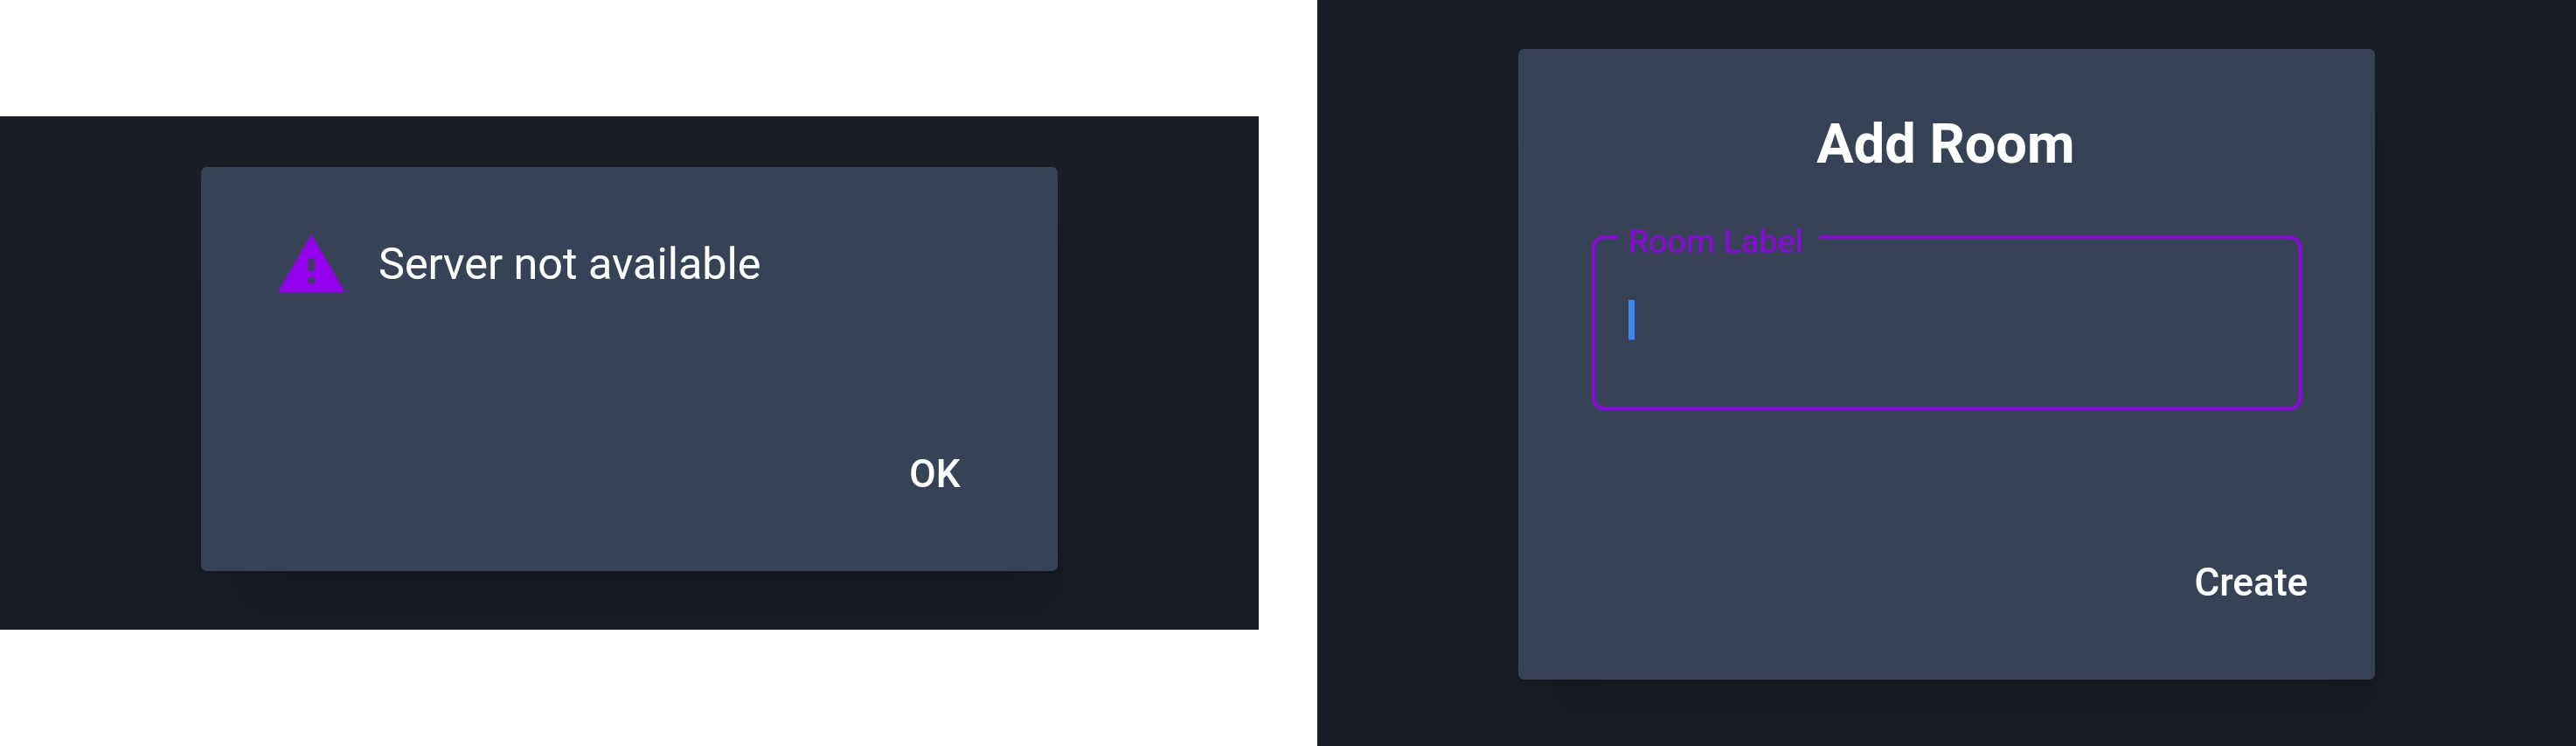
\includegraphics[width=\textwidth]{images/app_dialog.png}
	\centering
	\caption{Dialog Widgets}
	\label{fig:app_dialog}
\end{figure}

Unter den Listen-Widgets sind zum einen allgemeine Listen, die dem Design aus dem Entwurf der App entsprechen, und zum
anderen Listen für spezifische Modell-Klassen.
Diese Listen basieren auf den allgemeinen Listen.
So gibt es zum Beispiel Listen für Räume, Tracker oder auch die Schritte eines Workflows.
Die verschiedenen Listen sind in \autoref{fig:app_lists} zu sehen.

\begin{figure}[htbp]
	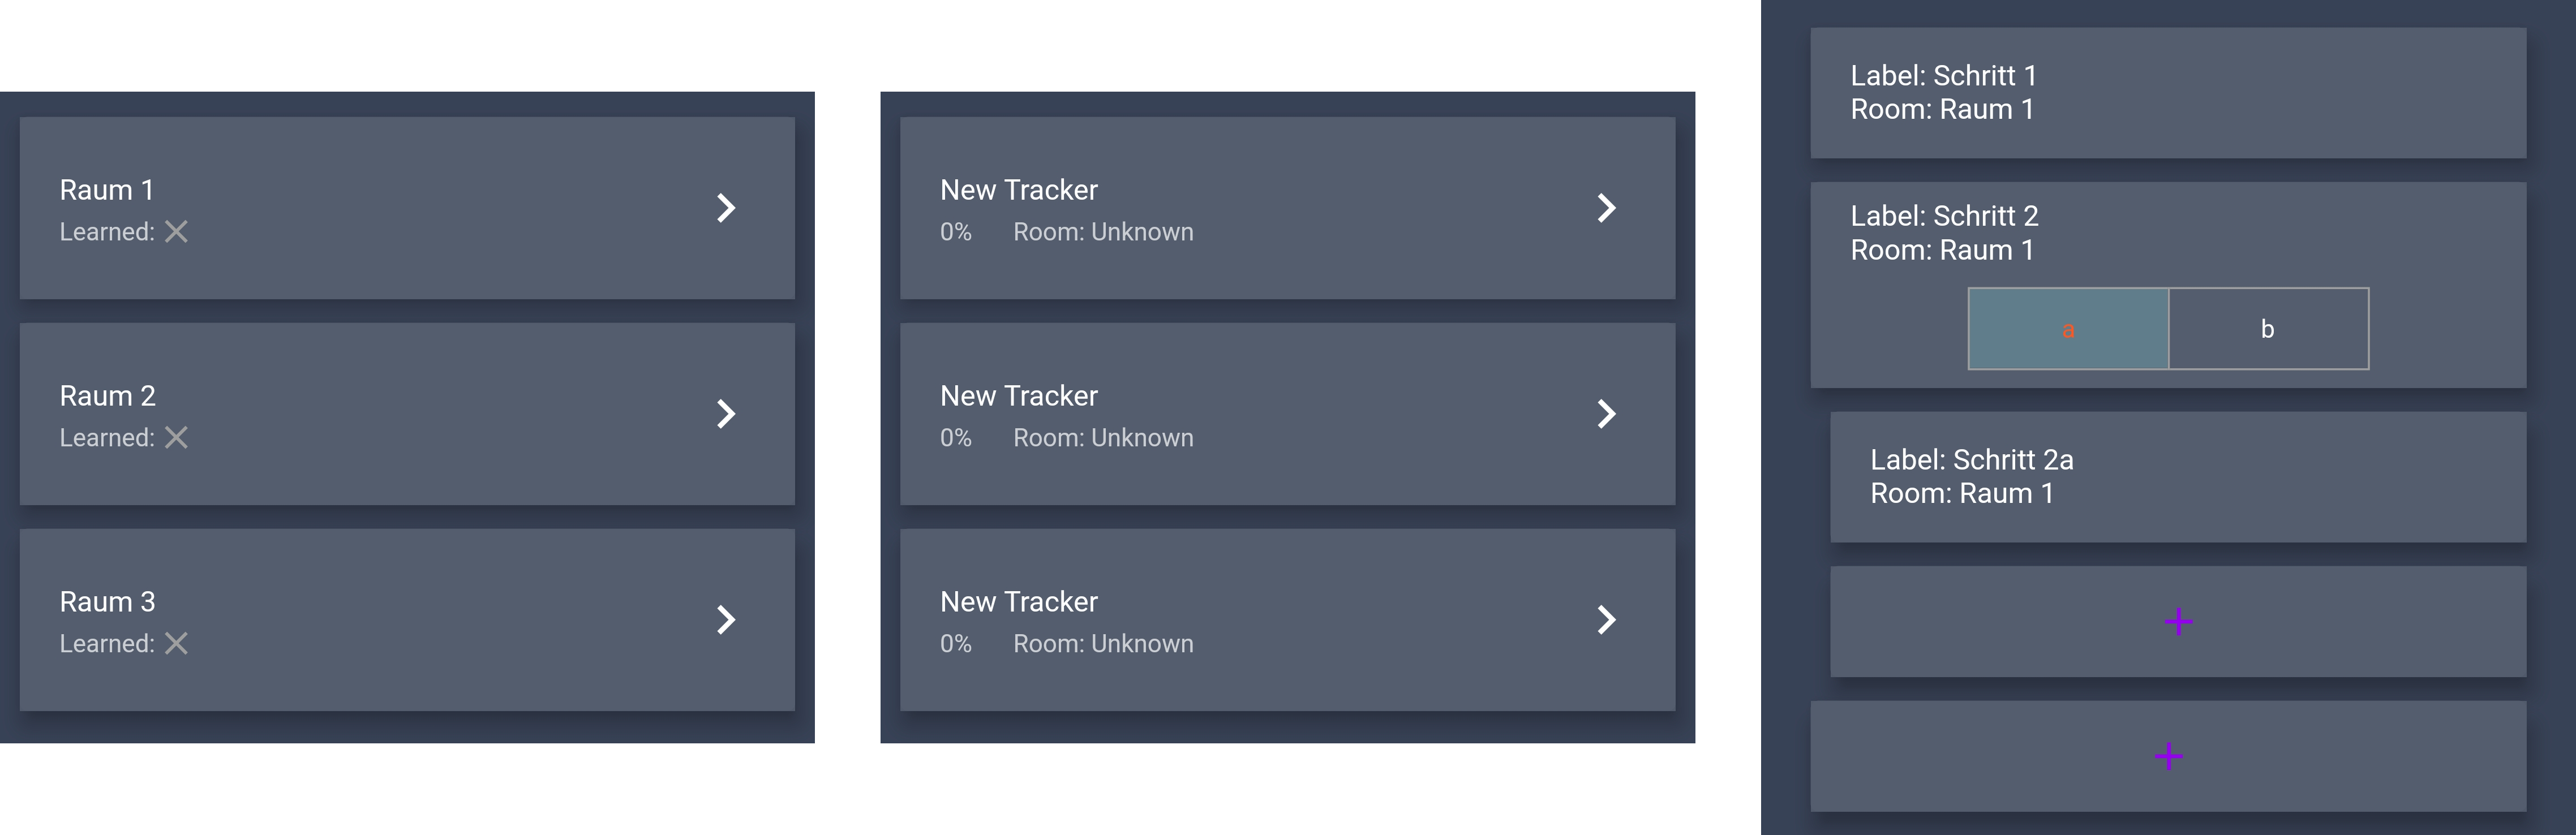
\includegraphics[width=\textwidth]{images/app_lists.png}
	\centering
	\caption{Listen Widgets}
	\label{fig:app_lists}
\end{figure}

Unter den allgemeinen Widgets gibt es zum Beispiel Auswahllisten oder ein Countdown.

Alle Widgets können Parameter entgegennehmen, die zur Übergabe von Einstellungen für dieses Widget oder als Rückgabe
von Informationen dienen können.
Als Rückgabe werden meistens entweder sogenannte \enquote{Callback}-Funktionen oder \enquote{Controller} verwendet.
Callback-Funktionen sind Funktionen von zum Beispiel der Seite, die das Widget verwendet, die dem Widget als Parameter
mitgegeben werden.
Möchte das Widget Informationen zurückgeben, wird der entsprechende Callback aufgerufen und als Parameter die eigentliche
Funktion mitgegeben.
Verwendet das Widget einen Controller wird dem Widget ein Objekt mitgegeben, welches die zu verschickenden
Informationen speichern kann.
Da dem Widget selbst nur eine Referenz des Objektes mitgegeben wird, kann das Widget neue Informationen einfach in dieses
Controller-Objekt schreiben.

\section{Hardware-Gehäuse}

Neben der Hardware des spezifischen Trackers und der Software wurde auch ein Hardware-Gehäuse entwickelt.
Dieses Gehäuse soll den Tracker mit der Batterie beinhalten und eine Möglichkeit bieten, dieses an einem Stapel Papier zu befestigen.
Die Herstellung des Gehäuses soll in einem 3D-Drucker erfolgen.
Dazu muss das Gehäuse digital modelliert werden.

Bevor die Modelle selbst erstellt werden können, muss ein grobes Layout vorliegen.
Für den Paper-Tracker wurden zwei verschiedene Layouts in Betracht gezogen.
Diese werden in den folgenden Sektionen genauer erläutert und die aus den Layouts entstandenen Modelle gezeigt.

\subsection{Layout Controller auf der Batterie}
Das erste Layout ist in \autoref{fig:case-lay-on} abgebildet.
Bei diesem Layout befindet sich der Mikrocontroller auf der Batterie.

\begin{figure}[htbp]
	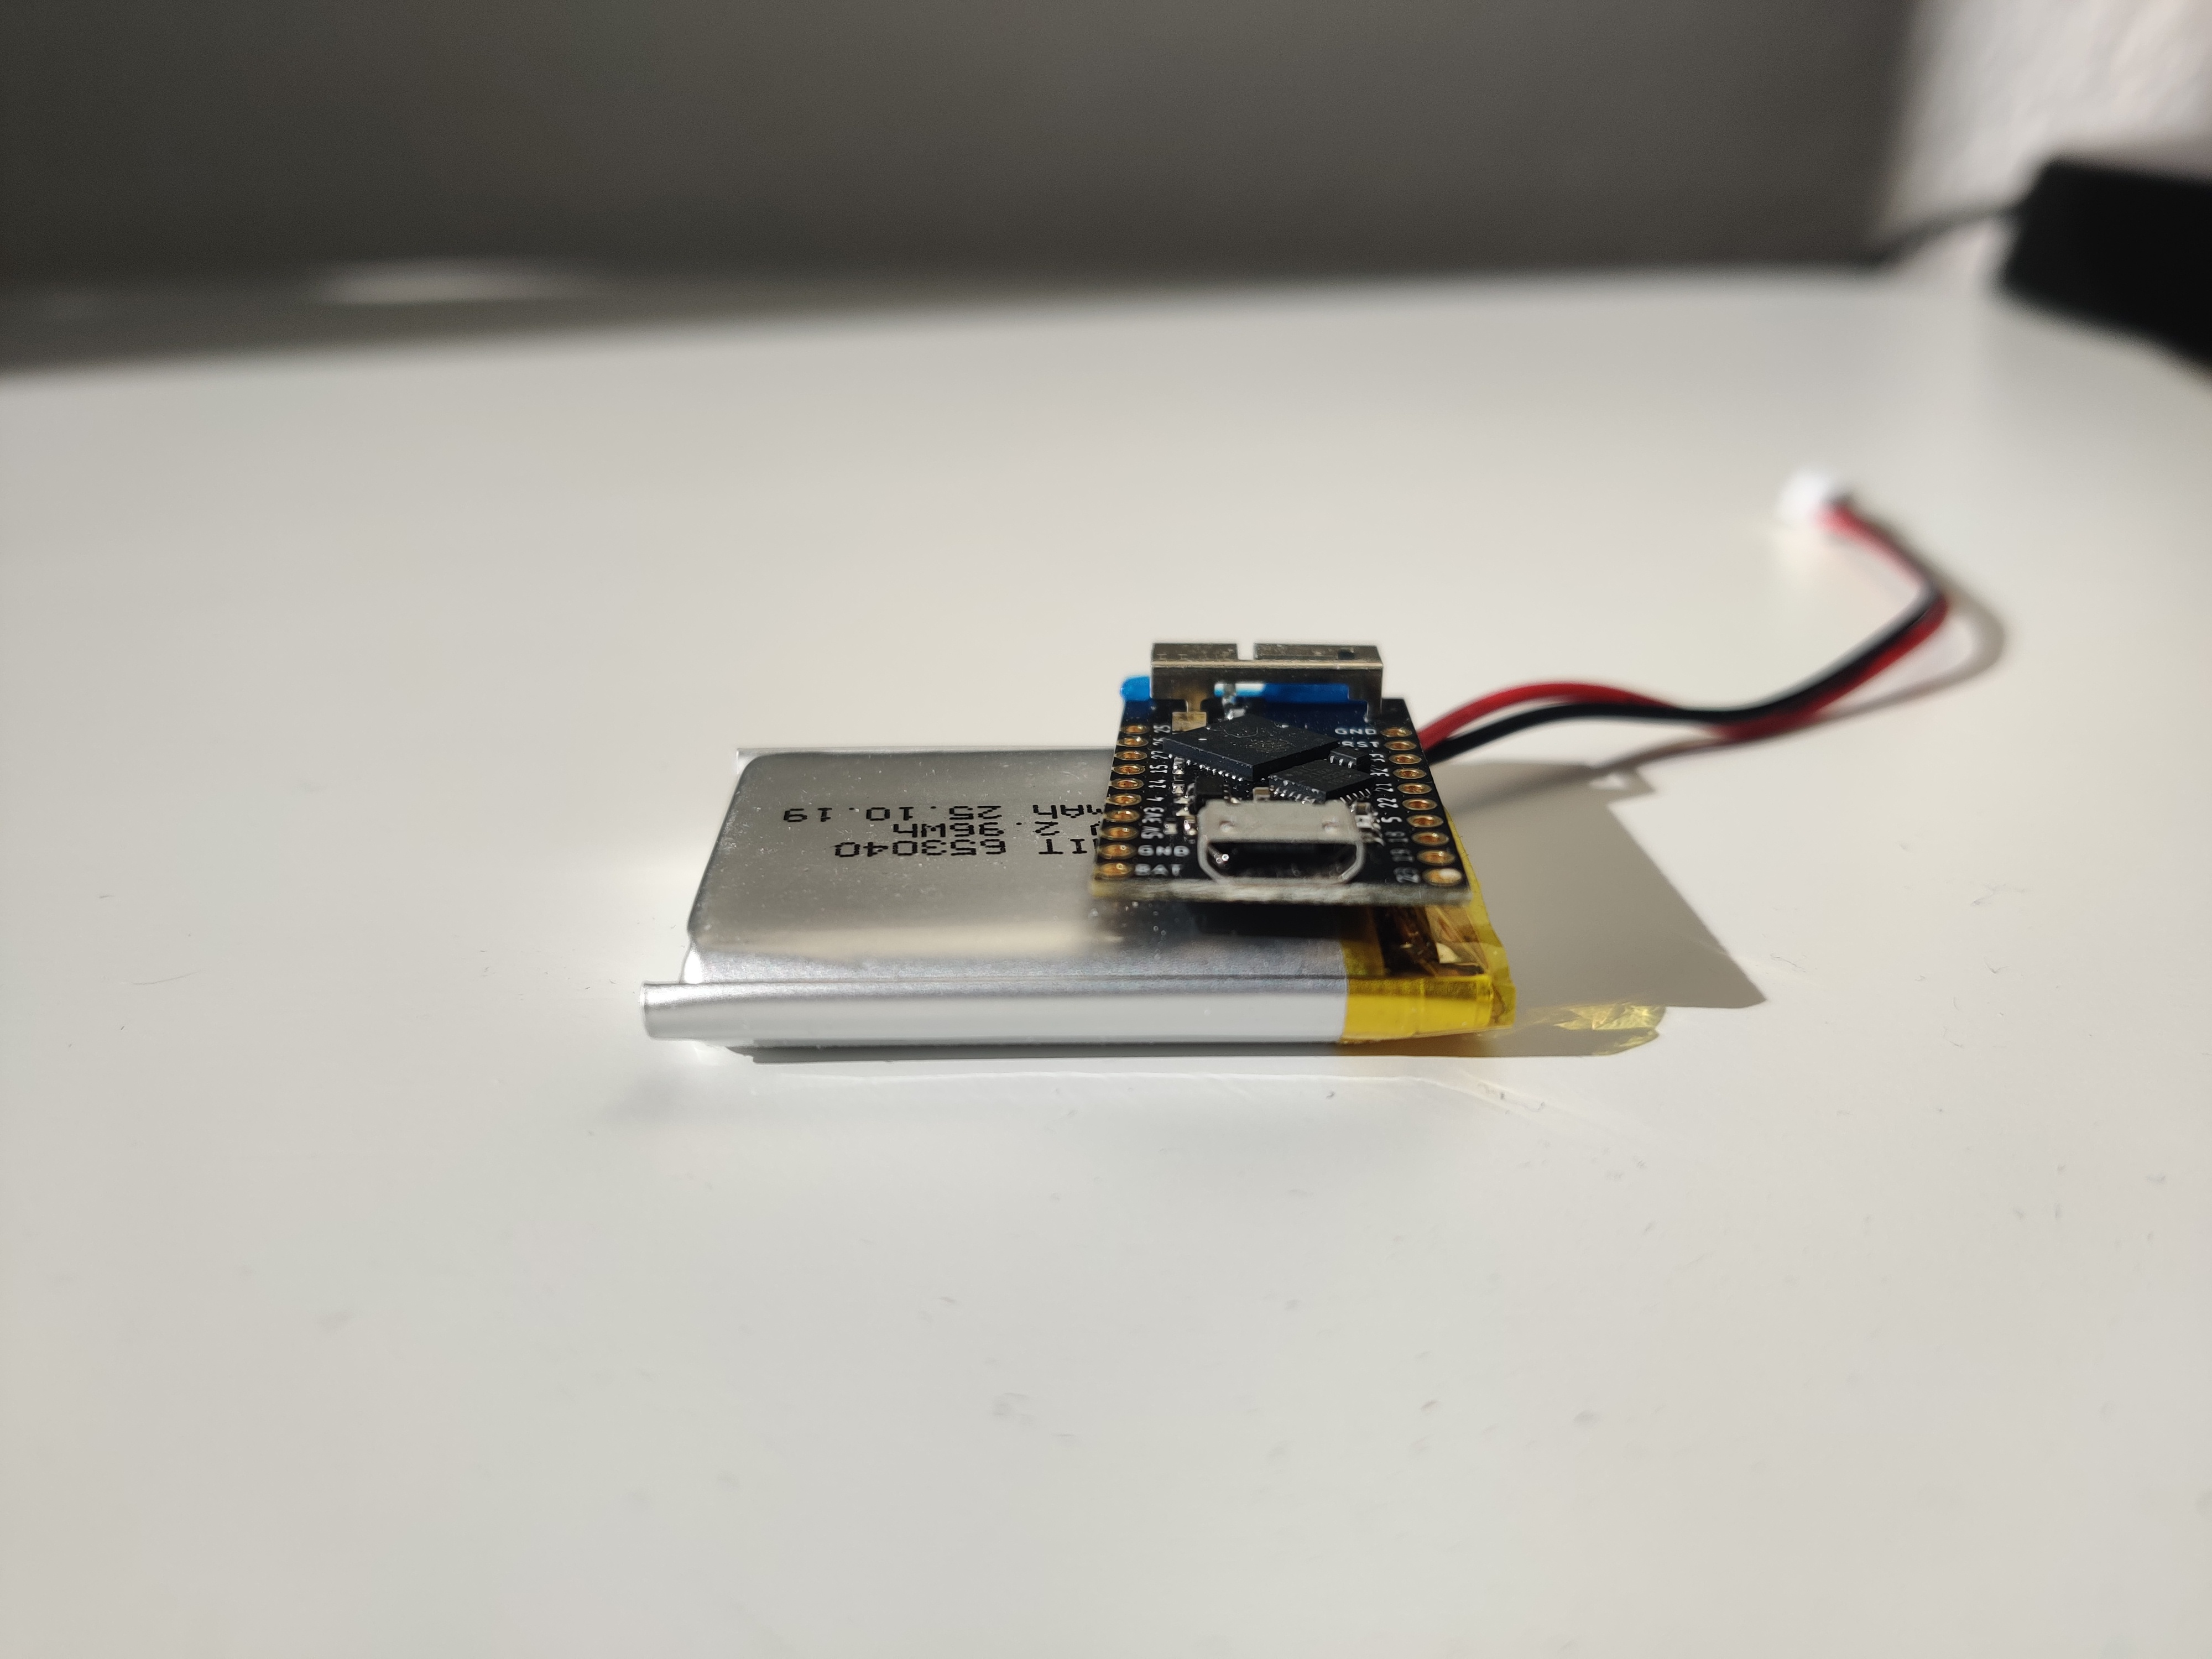
\includegraphics[width=300px]{images/case/pico_on_battery.jpg}
	\centering
	\caption{Gehäuse-Layout mit Mikrocontroller auf der Batterie}
	\label{fig:case-lay-on}
\end{figure}

Dies ergibt den Vorteil, dass die Grundfläche des Trackers mit ca. 45x35mm sehr gering gehalten wird.
Daraus ergibt sich dementsprechend der Nachteil, dass mit ca. 15mm die Konstruktion relativ hoch wird.

Das aus dem Layout entstandene Modell besteht aus zwei verschiedenen Teilen: Dem Körper des Gehäuses und dem Deckel.

Der Körper ist in \autoref{fig:case-high-body} dargestellt.
Er bietet eine Art Schublade, in welche die Batterie hineinpasst.
Oberhalb der Schublade wird der Mikrocontroller durch Wände am Platz gehalten.
An der Seite gibt es eine Aussparung, um den \gls{USB}-Port zum Laden benutzen zu können.

Geschlossen wird der Körper mit dem Deckel.
Dies ist in \autoref{fig:case-high} dargestellt.
Die beiden Teile sollen nur über das Zusammenstecken miteinander verbunden werden.
Am Deckel ist auch der Mechanismus zum Anklemmen des Gehäuses an Papier angebracht.
Er besteht aus einem Steg, der schräg zum Gehäusekörper zeigt.
Zudem sind Noppen angebracht, die die Grifffestigkeit erhöhen sollen.

\begin{figure}[htbp]
	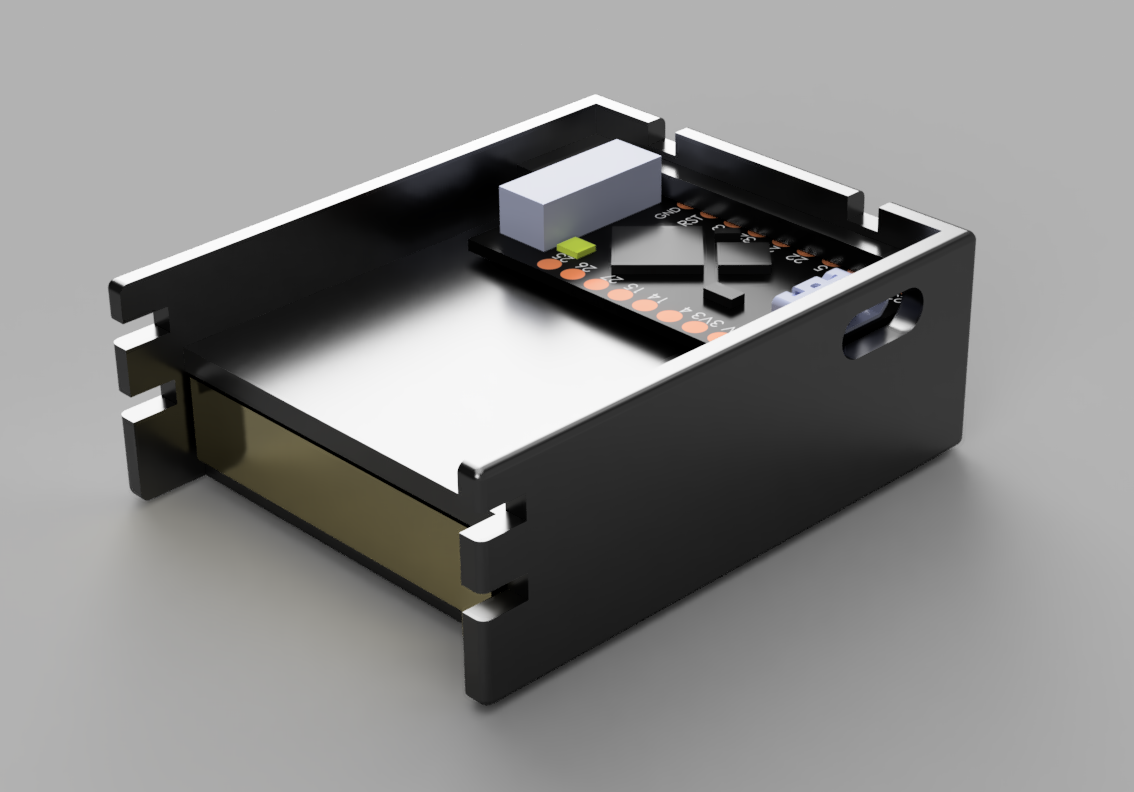
\includegraphics[width=300px]{images/case/high_body.png}
	\centering
	\caption{Körper des Gehäuse-Modells mit Controller auf der Batterie}
	\label{fig:case-high-body}
\end{figure}

\begin{figure}[htbp]
	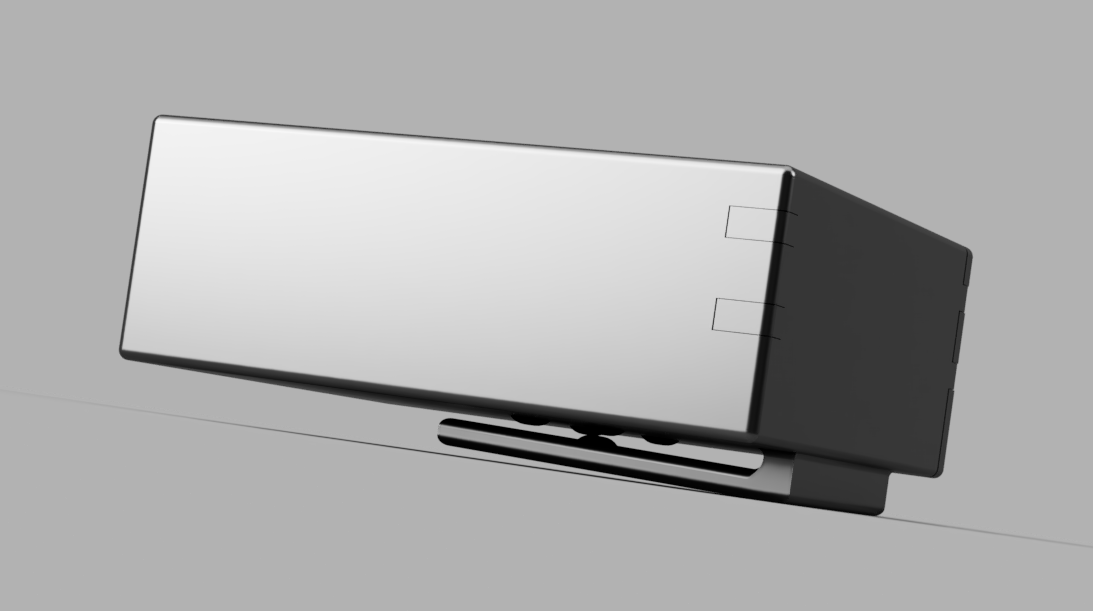
\includegraphics[width=300px]{images/case/high_complete.png}
	\centering
	\caption{Gehäuse-Modells mit Controller auf der Batterie}
	\label{fig:case-high}
\end{figure}

\FloatBarrier

\subsection{Layout Controller neben der Batterie}
Das zweite Layout ist in \autoref{fig:case-lay-beside} abgebildet.
Der Unterschied zum ersten Layout ist, dass der Mikrocontroller neben der Batterie platziert wird.

\begin{figure}[htbp]
	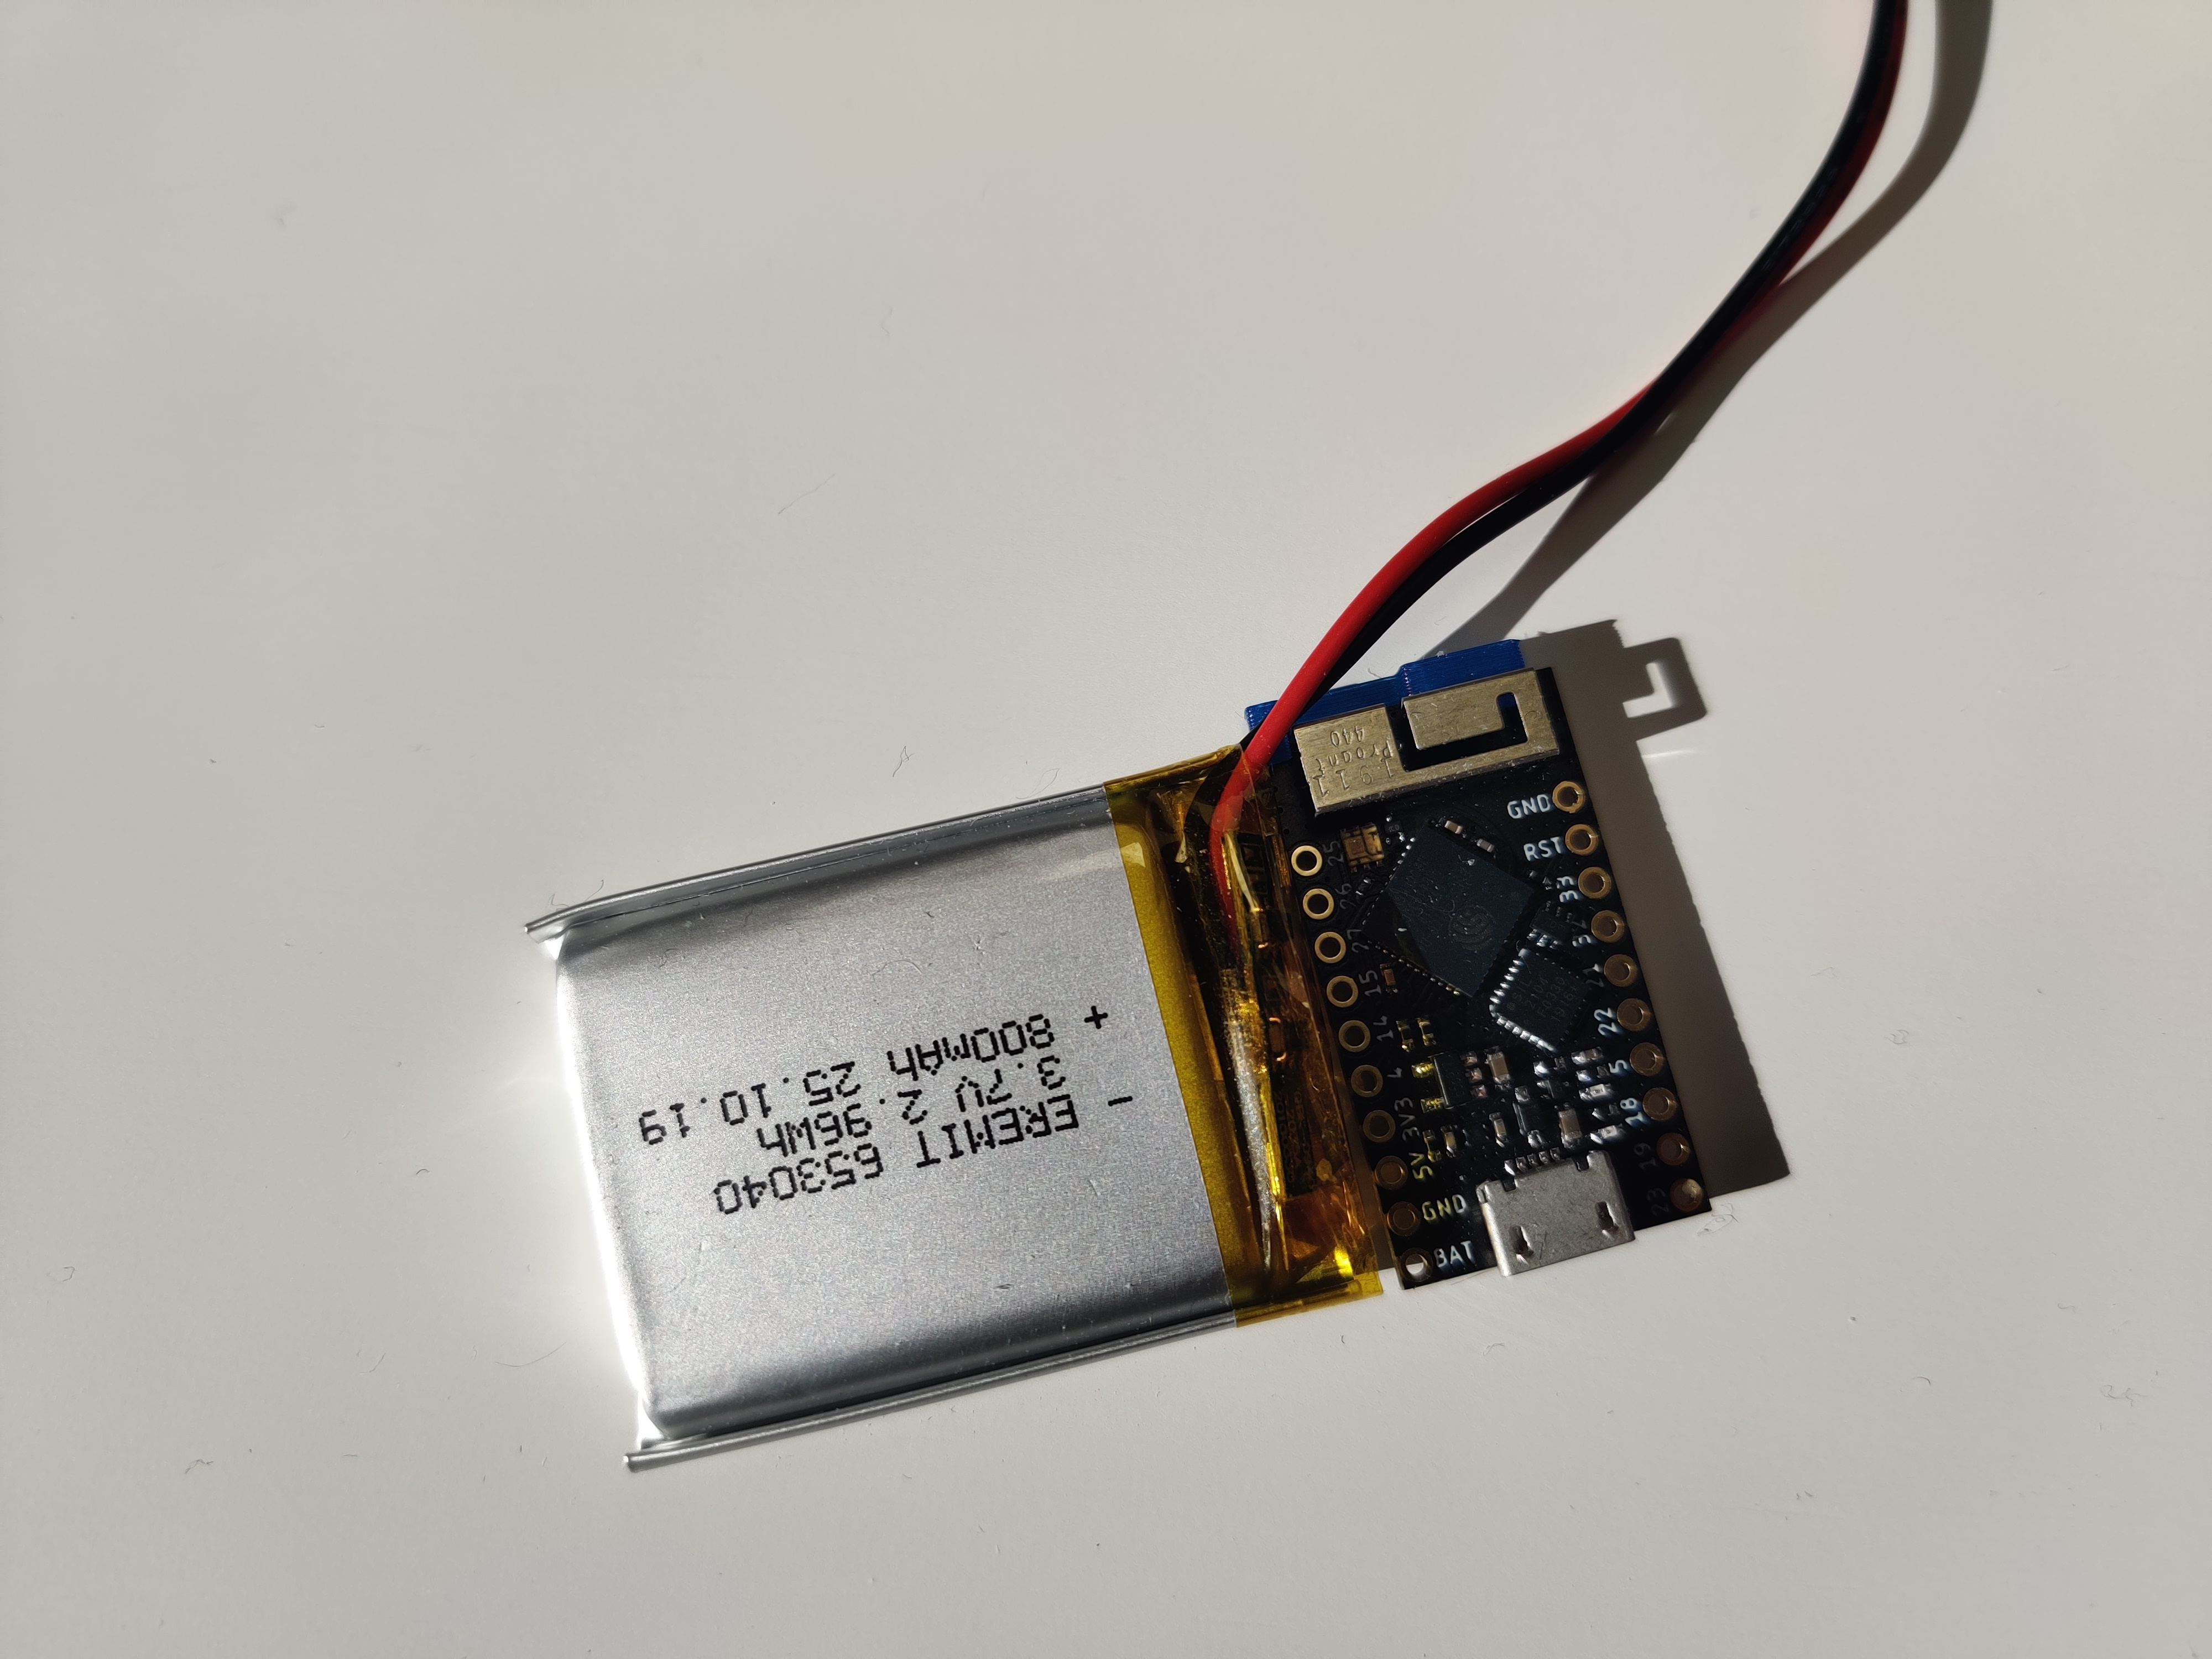
\includegraphics[width=300px]{images/case/pico_beside_battery.jpg}
	\centering
	\caption{Gehäuse-Layout mit Mikrocontroller neben der Batterie}
	\label{fig:case-lay-beside}
\end{figure}

Dies resultiert in einer erhöhten Grundfläche zum ersten Layout von 70x35mm, aber in einer Reduktion der Höhe auf nur 12mm.

Das Modell nach diesem Layout ist in drei verschiedene Teile aufgeteilt.
Es gibt, wie beim ersten Layout, auch einen Körper und einen Deckel.
Zusätzlich gibt es jedoch noch den Clip zum Befestigen an Papier.
Dieser ist demnach nicht mehr im Deckel mit enthalten.

Der Körper ist in \autoref{fig:case-low-body} dargestellt.
Er bietet Platz für die Batterie und den Mikrocontroller nebeneinander.
Für den \gls{USB}-Port ist ebenfalls in der Außenwand eine Aussparung vorhanden.
Kleine Erhebungen halten die Teile am Platz und verhindern ein Umherschieben.
In diesen Erhebungen sind auch Löcher für Schrauben inkludiert und auf der Unterseite Platz für eine Mutter.
Der größere Einschnitt in der Unterseite ist für den Clip bestimmt.

\begin{figure}[htbp]
	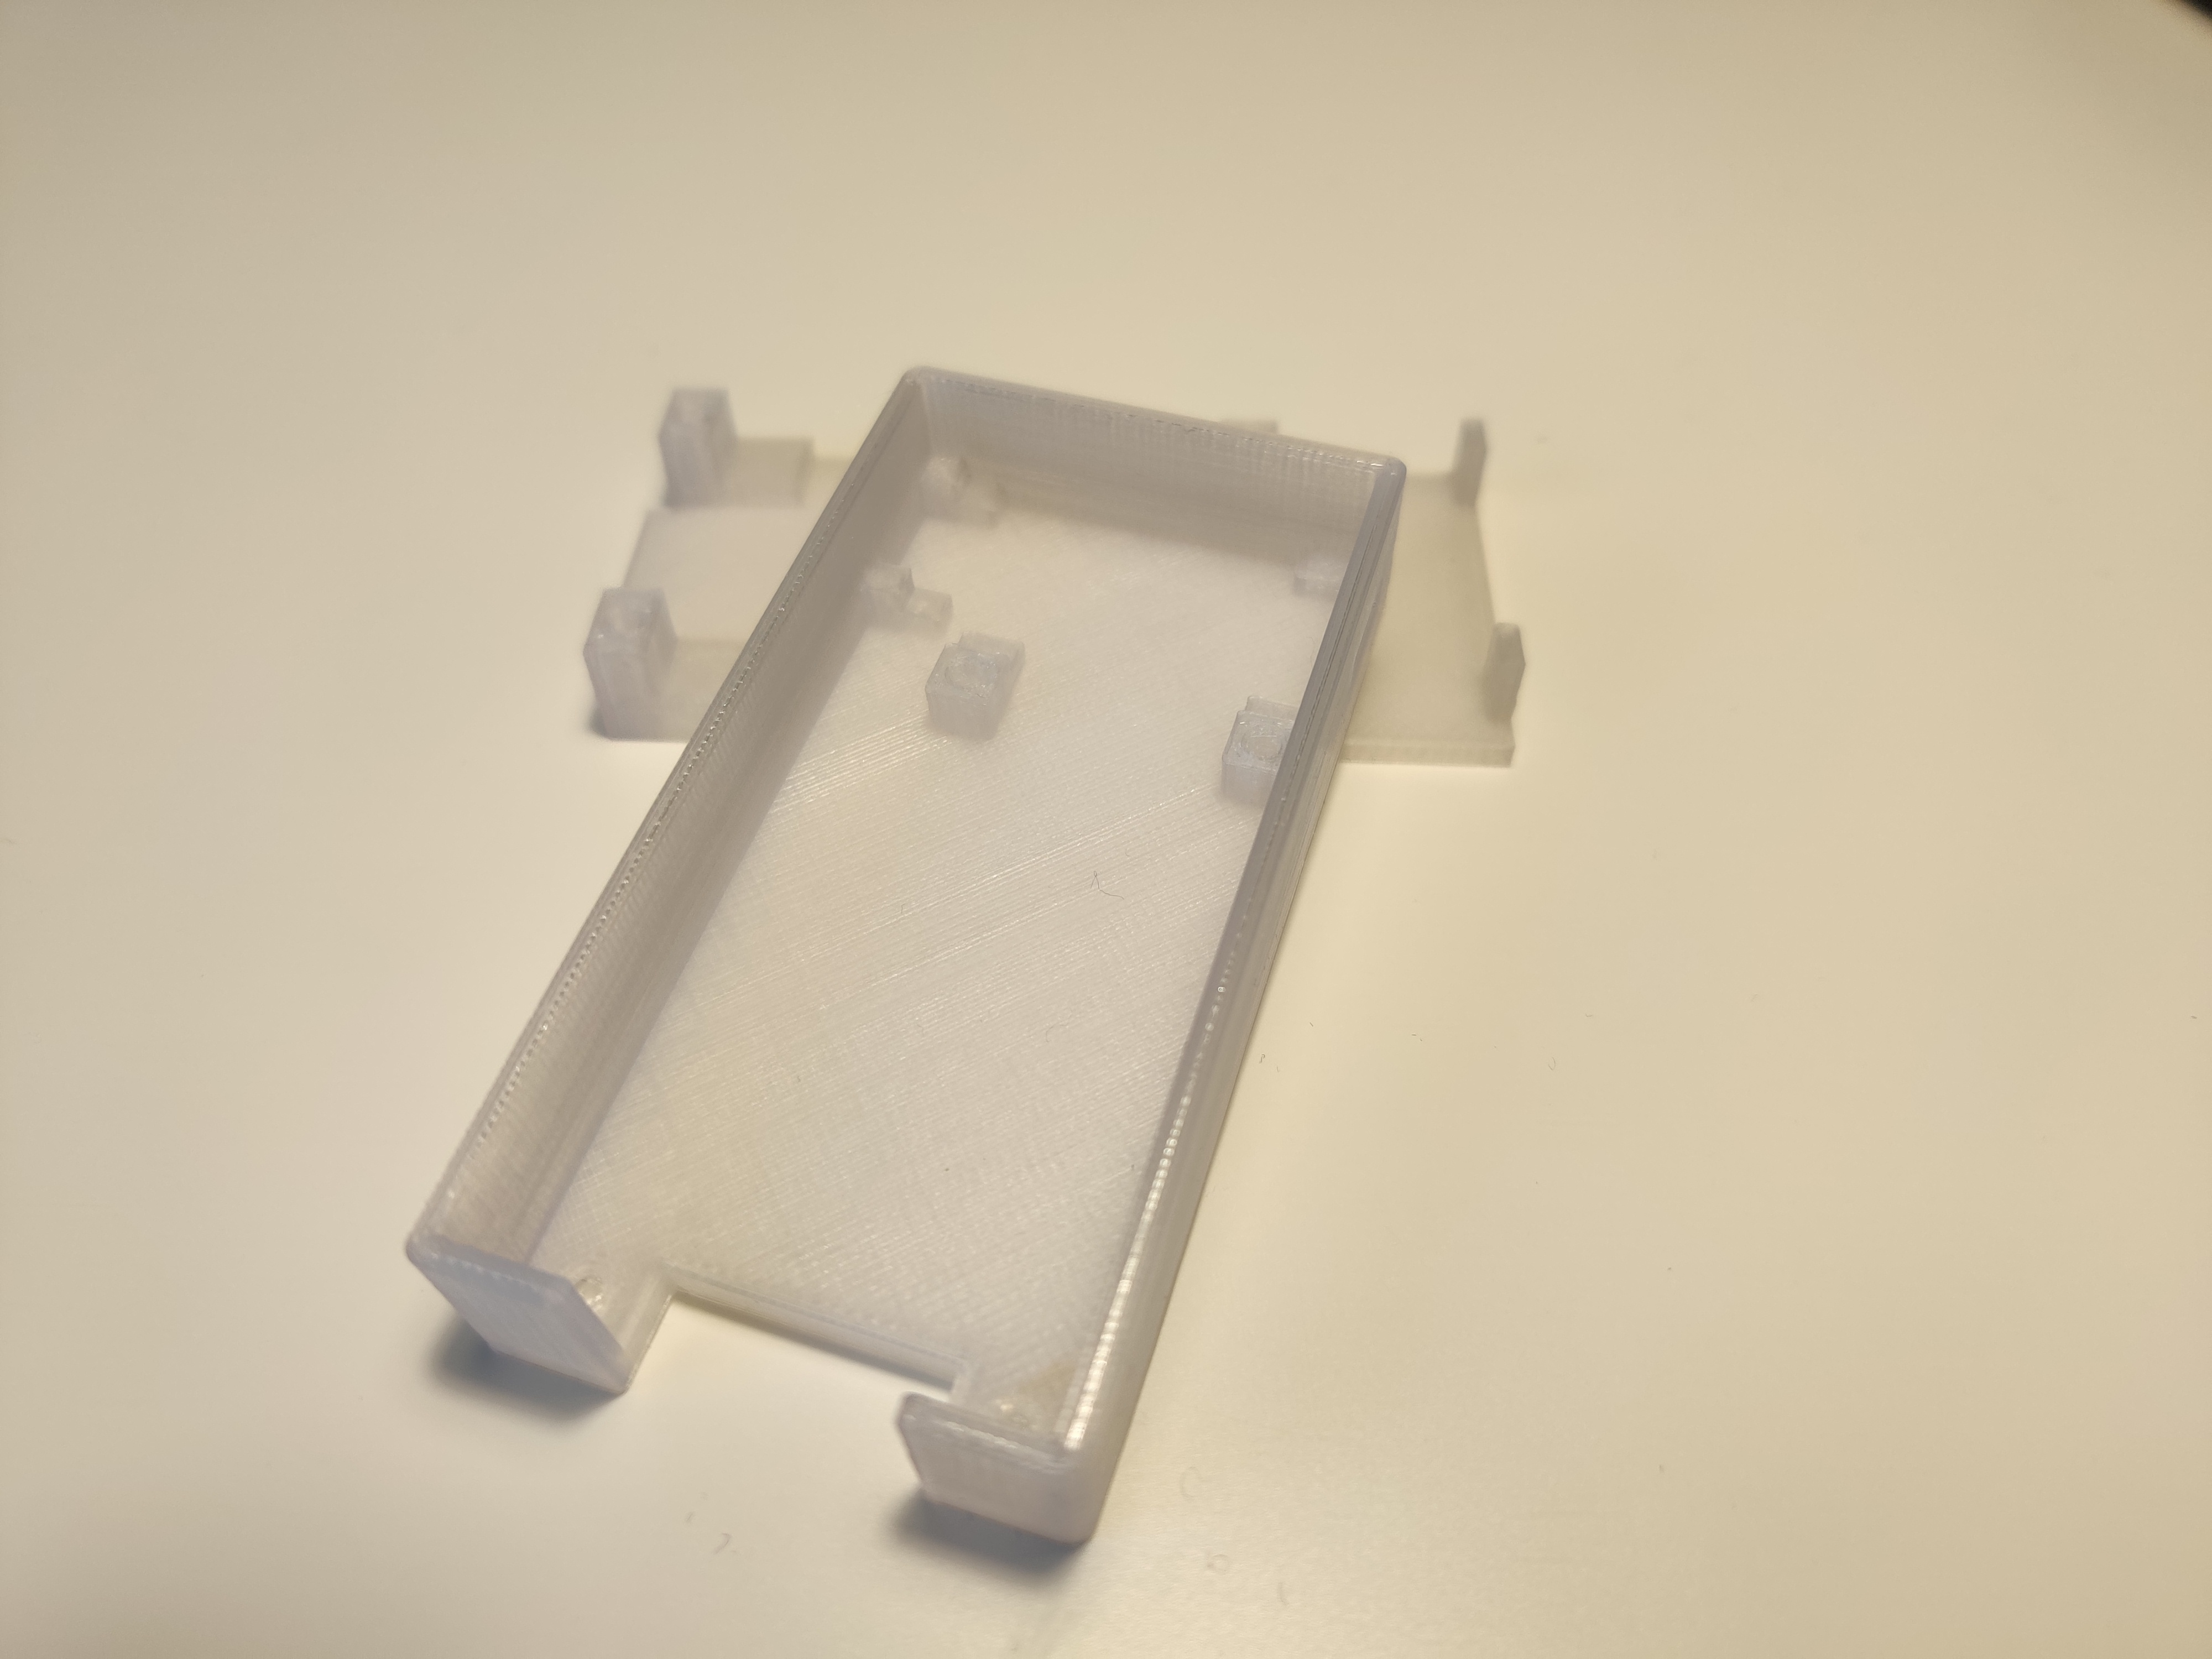
\includegraphics[width=300px]{images/case/low_body.jpg}
	\centering
	\caption{Körper des s mit Controller neben der Batterie}
	\label{fig:case-low-body}
\end{figure}

Der Deckel des Modells ist ähnlich dem Körper, besitzt aber keine Außenwände.
Er ist in \autoref{fig:case-low-lid} abgebildet.
Die kleinen Erhebungen des Deckels fixieren die Teile innerhalb des Gehäuses auf der vertikalen Achse.
Statt Platz für eine Mutter auf der Außenseite der Erhebungen mit Schraubenlöchern, ist eine Einsenkung für den Schraubkopf vorgesehen.

\begin{figure}[htbp]
	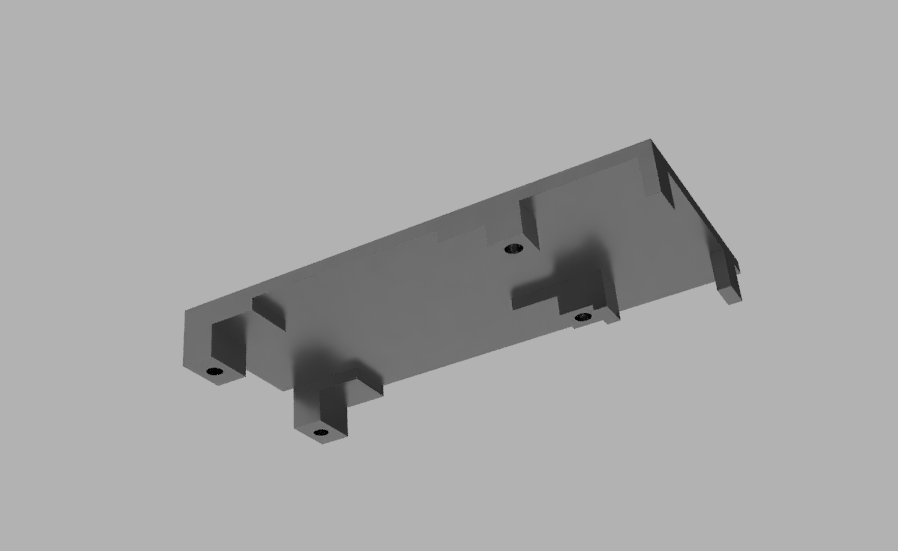
\includegraphics[width=300px]{images/case/low_lid.png}
	\centering
	\caption{Deckel des Gehäuse-Modells mit Controller neben der Batterie}
	\label{fig:case-low-lid}
\end{figure}

Angebracht ist der Clip an dem Einschnitt im Körper und fixiert durch die zwei danebenliegenden Schraubenlöcher.
Die Schraube wird dabei zwischen den Erhebungen des Körpers und des Deckels, sowie durch die in
\autoref{fig:case-low-clip} dargestellten Flügel des Clips geführt.
Für die Fixierung an einem Papierstapel wurde die gleiche Technik wie für das erste Layout verwendet.
Um den 3D-Druck zu simplifizieren wurden bei diesem Entwurf jedoch keine Noppen an den Clip und an
den Körper des Gehäuses angebracht. Diese werden nach dem Druck aufgeklebt.

\begin{figure}[htbp]
	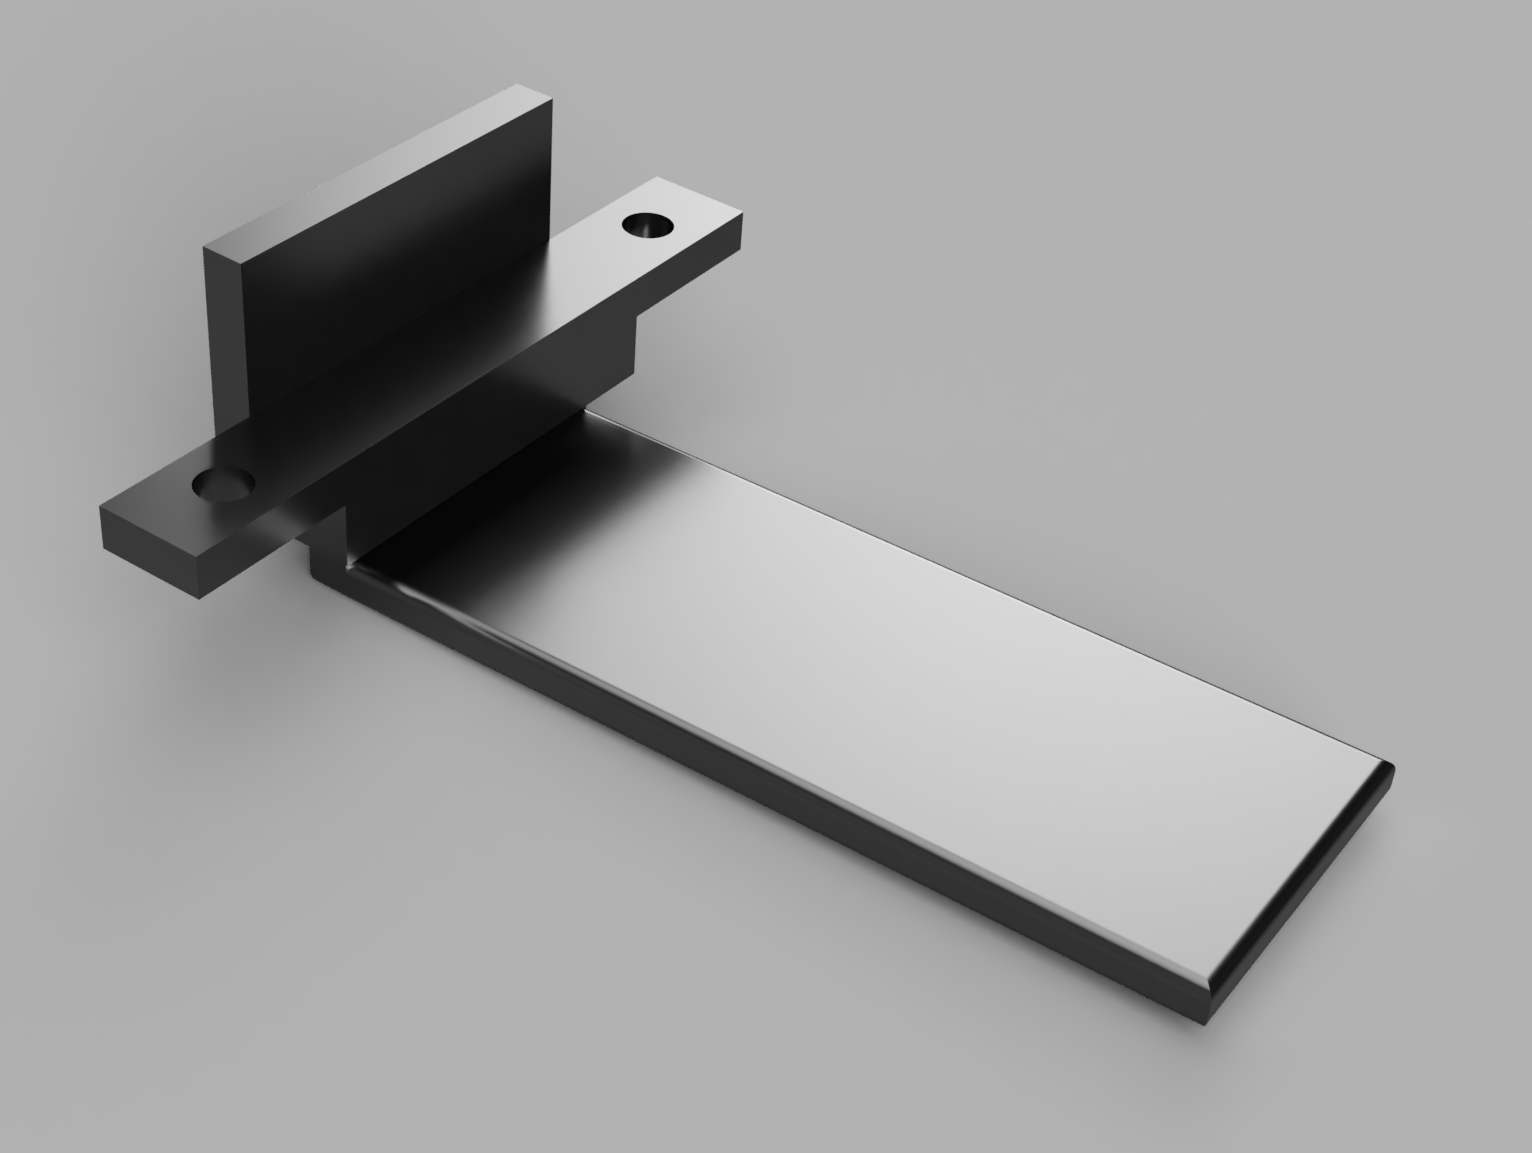
\includegraphics[width=300px]{images/case/low_clip.png}
	\centering
	\caption{Clip des Gehäuse-Modells mit Controller neben der Batterie}
	\label{fig:case-low-clip}
\end{figure}

\section{Bestehende Herausforderungen}

Es konnte zwar eine funktionierende und fast vollständige Lösung implementiert werden, die jedoch noch ein paar
Herausforderungen beinhaltet.
Dies sind mehrere Anpassungen oder Fehler, die aufgrund der begrenzten Projektzeit nicht angegangen werden konnten.

\subsection{\glsentrylong{UI}-Details in der App} \label{sec:impl-challenges-ui}

Innerhalb der App für den Paper-Tracker gibt es eine fehlende Funktion, die noch nicht implementiert wurde.
Dies ist die Unterstützung für mehrere Räume pro Schritt in einem Workflow Template.
Aktuell kann nur ein Raum ausgewählt werden, der immer in einer eigenen Liste an erster Stelle an den Server geschickt wird.
Konkret müssten auf der \enquote{WorkflowTemplatePage} und den dazugehörigen Widgets alle Auswahllisten für einen Raum durch
eine Mehrfachauswahl ersetzt werden.
Weiter müsste das Widget für die Darstellung von Steps eines Templates so angepasst werden, dass es
mehrere Räume anzeigen kann.

Zusätzlich zu dieser funktionalen Änderung, sollten einige nichtfunktionale Änderungen durchgeführt werden.
Zum einen muss das Farbschema der App überarbeitet werden.
Der Kontrast zwischen dem Violett und verschiedenen Hintergrundfarben liegt lediglich zwischen $1.21:1 - 1.68:1$.
Empfohlen wird laut dem Kriterium 1.4.3 in \cite{W3C2018} ein Kontrastwert von mindestens $4.5:1$.
Auch weitere verwendete Farben sind schwer erkennbar und können durch bessere ersetzt werden.

Die Mehrfachauswahl der für das Einlernen eines Raumes verwendeten \gls{SSID}s besitzt einen kleinen Fehler, der jedoch
für den Benutzer sehr verwirrend sein kann.
Es ist möglich die Auswahlbox eines Eintrages der Liste durch Drücken auf den gesamten Eintrag zu setzen, jedoch nicht
bei einem Druck auf die Auswahlbox selbst.
Dies kann dem Nutzer suggerieren, dass er keine Auswahl treffen kann, da meistens versucht wird, mit der Auswahlbox selbst
zu interagieren.

Zum Schluss exisitiert noch eine Inkonsistenz in der Nutzung von Textfeldern innerhalb der App.
Bei einigen Textfeldern, zum Beispiel in dem Dialog zum Erstellen eines Raumes, ist der Text der letzten Eingabe vorausgefüllt.
In anderen Textfeldern ist dies nicht der Fall und das Feld ist bei jedem Öffnen des Dialogs leer.
Hier muss sich auf ein konsistentes Verhalten geeinigt werden und dieses konsequent in der App umgesetzt werden.

\subsection{Messung des Batteriestandes}

Wie in \autoref{sec:hardware-used-technologies} beschrieben, stellt die TinyPICO-Plattform eine
Bibliothek bereit, mit der die Spannung des \gls{Akku}s abgefragt werden kann und somit der aktuelle
Ladestand berechnet werden kann. Diese Information ist wertvoll, um zu verhindern, dass ein Workflow
nicht richtig getracked wird, weil der \gls{Akku} eines Trackers leer wird. Daher wird der
Ladestand, wie in \autoref{tab:detail-attributes} gezeigt, auch in der App dargestellt. Dies macht das
Überprüfen des Ladestandes sehr komfortabel.

Problematisch ist jedoch, dass die Spannung des \gls{Akku}s nur sehr grob gemessen wird, was dazu
führt, dass der Tracker bei zwei direkt hintereinander durchgeführten Abfragen des Ladestandes mit
Schwankungen bis zu $5\%$ antwortet. Dieses Hindernis lässt sich durch weitere Hardware, welche
die Spannung misst, überwinden. Dies würde den Tracker weiter vergrößern, weswegen diese Option
nicht in Frage kommt. Eine weitere mögliche Lösung könnte eine Filterung nach mehreren Messungen
sein. Diese könnte auf Seiten des Trackers oder im Server implementiert werden.

Auch der Ladestatus, also ob ein Tracker aktuell aufgeladen wird oder sich entlädt, wird von der
gelieferten Bibliothek nicht immer korrekt wiedergegeben. Dies kann dazu führen, dass ein sich
entladender Tracker in der App vorübergehend als ladend angezeigt wird. Auch für die Korrektur dieses
Fehlers wäre externe Hardware nötig. Anders als das vorherig beschriebene Problem kann hierfür kein
Filter genutzt werden, da auch mehrere hintereinander durchgeführte Abfragen des Status sehr häufig zum
gleichen Ergebnis führen, auch wenn dieses falsch ist.

\subsection{Weitere Verkleinerung des Trackers}

Es konnte mit dem ausgewählten Mikrocontroller und der Batterie schon ein kompakter Tracker erreicht werden.
Trotzdem wäre mit einer weiteren Optimierung durch zum Beispiel einem für das Projekt angepassten \gls{PCB}
oder einer kleineren Batterie in Kombination mit reduziertem Stromverbrauch ein noch kompakterer Tracker möglich.
